%==================================================================
% Ini adalah bab 4
% Silahkan edit sesuai kebutuhan, baik menambah atau mengurangi \section, \subsection
%==================================================================

\chapter[HASIL PENELITIAN DAN PEMBAHASAN]{\\ HASIL PENELITIAN DAN PEMBAHASAN}

\section{Hasil Penelitian}

\subsection{Pengembangan Sistem Informasi}
Pengembangan sistem informasi organisasi INFINITE dilakukan dengan menggunakan model pengembangan perangkat lunak \textit{Waterfall}, dengan tahapan sebagai berikut:

\subsubsection{\textit{Requirements Definition}}

Pada tahap pendefinisian kebutuhan, dilakukan analisis kebutuhan melalui wawancara dengan Presiden INFINITE dan Ketua Divisi \textit{Research and Development}, serta observasi terhadap sistem informasi organisasi yang telah ada sebelumnya. Dari kegiatan tersebut, diperoleh informasi penting sebagai berikut:

\begin{enumerate}
      \item Sistem informasi organisasi INFINITE sebelumnya terdiri dari dua sistem terpisah, yaitu sistem berbasis Laravel dan sistem berbasis CMS Strapi. Kedua sistem ini tidak terintegrasi, sehingga data tersebar di dua basis data yang berbeda.
      \item Sistem sebelumnya tidak memiliki autentikasi terpusat, sehingga pengguna harus melakukan pendaftaran dan masuk secara terpisah di masing-masing sistem.
      \item Sistem sebelumnya tidak memiliki manajemen peran dan izin akses yang memadai, sehingga kontrol akses terhadap fitur-fitur sistem tidak konsisten.
      \item Sistem berbasis Laravel sebelumnya memiliki fitur pengelolaan data anggota, kompetisi, tim, prestasi, dan pengajuan pendanaan, namun tidak memiliki fitur manajemen konten seperti testimoni dan galeri proyek, serta manajemen struktur pengurus organisasi.
      \item Sistem berbasis CMS Strapi sebelumnya memiliki fitur manajemen konten dan struktur pengurus organisasi, namun tidak memiliki fitur pengelolaan data anggota dan tidak terintegrasi dengan sistem berbasis Laravel.
\end{enumerate}

Hasil analisis kebutuhan kemudian digunakan sebagai dasar penentuan spesifikasi sistem informasi INFINITE.

\begin{enumerate}[listparindent=1cm]
      \item Analisis Kebutuhan Fungsional

            Berdasarkan hasil wawancara dan observasi, kebutuhan fungsional sistem informasi organisasi INFINITE mencakup fitur-fitur utama yang diperlukan untuk mendukung pengelolaan data organisasi secara terintegrasi. Sistem informasi terdiri dari dua komponen utama yang saling terintegrasi, yaitu \textit{backend} API Laravel dan \textit{frontend} Next.js. Sistem ini mendukung autentikasi terpusat melalui protokol \textit{OpenID Connect} (OIDC) dengan sistem \textit{Single Sign-On} (SSO) INFINITE. Fitur-fitur yang dikembangkan meliputi:

            \begin{enumerate}[label=\alph*.]
                  \item Pengelolaan data anggota, meliputi data profil personal (nama, NIM, strata, fakultas, program studi), data kontak (telepon, email), serta data keanggotaan (persona, tanggal mulai dan berakhir keanggotaan, status aktif, dan status istimewa).
                  \item Pengelolaan data kepengurusan, meliputi pengurus inti organisasi beserta divisi dan anggotanya, serta pengurus komunitas beserta anggotanya.
                  \item Pengelolaan data kompetisi, meliputi katalog kompetisi, pelaksanaan kompetisi spesifik, tipe penyelenggara, tingkat kompetisi, peringkat, durasi kompetisi, jenis luaran, serta tipe tim.
                  \item Pengelolaan data tim perlombaan, meliputi pembentukan tim oleh anggota, penunjukan ketua tim, serta keanggotaan tim.
                  \item Pengelolaan pengajuan pendanaan oleh tim, meliputi pengunggahan dokumen bukti lolos kompetisi dan proposal pendanaan, dengan alur persetujuan.
                  \item Pencatatan prestasi yang diraih oleh tim, dengan perhitungan poin berdasarkan pembobotan multi-dimensi dari enam taksonomi kompetisi.
                  \item Papan peringkat pencapaian anggota yang dihitung secara agregat per tahun berdasarkan total poin prestasi.
                  \item Pengelolaan testimoni dari alumni tentang dampak INFINITE terhadap karier mereka, serta testimoni proyek yang pernah dikerjakan oleh anggota.
                  \item Pengelolaan galeri proyek yang mendokumentasikan proyek-proyek yang telah dikerjakan oleh anggota.
                  \item Pengelolaan data referensi akademik berupa strata, fakultas, dan program studi.
                  \item Manajemen peran dan izin akses untuk mengatur hak akses pengguna terhadap setiap fitur sistem.
                  \item Pengelolaan konfigurasi sistem berupa pengaturan kunci-nilai untuk parameter seperti periode registrasi ulang, tautan media sosial, dan pengaturan lainnya.
                  \item Penyediaan API untuk integrasi dan konsumsi oleh \textit{frontend}, \textit{landing page}, maupun sistem eksternal.
            \end{enumerate}

      \item Analisis Kebutuhan Non-Fungsional

            Kebutuhan non-fungsional sistem informasi organisasi INFINITE mencakup kebutuhan lingkungan pengembangan dan spesifikasi sistem sebagai berikut:

            \begin{enumerate}[label=\alph*.]
                  \item Kebutuhan Informasi Penunjang Sistem
                        \begin{itemize}
                              \item Konfigurasi sistem SSO INFINITE berbasis Authentik sebagai \textit{identity provider}.
                              \item Konfigurasi basis data PostgreSQL dan Redis Sentinel sebagai \textit{data store} untuk sistem.
                        \end{itemize}
                  \item Kebutuhan Spesifikasi Sistem
                        \begin{itemize}
                              \item Sistem dikembangkan dengan arsitektur \textit{headless}, memisahkan \textit{backend} API Laravel dari \textit{frontend} Next.js yang dihubungkan melalui antarmuka RESTful API.
                              \item \textit{Backend} menggunakan bahasa pemrograman PHP dengan kerangka kerja Laravel, basis data PostgreSQL, dan \textit{server} aplikasi Laravel Octane dengan FrankenPHP.
                              \item \textit{Frontend} menggunakan TypeScript dengan kerangka kerja Next.js (\textit{App Router}), Material UI (MUI) sebagai pustaka komponen, Tailwind CSS untuk utilitas gaya, Zustand untuk manajemen \textit{state}, dan Inversify untuk \textit{dependency injection}.
                              \item Sistem di-\textit{deploy} sebagai aplikasi terkontainerisasi di platform Kubernetes dengan pendekatan GitOps menggunakan ArgoCD.
                              \item Autentikasi menggunakan OIDC melalui sistem SSO INFINITE (Authentik) yang terintegrasi dengan \textit{library} better-auth pada \textit{frontend}.
                              \item Seluruh operasi CRUD tersedia melalui RESTful API berversi (\texttt{/api/v1/}) dengan \textit{cursor-based pagination}, penyaringan (\textit{filtering}), pengurutan (\textit{sorting}), dan pemuatan relasi (\textit{eager-loading}) menggunakan Spatie Query Builder.
                              \item Sistem mendukung penyimpanan berkas (\textit{blob}) dengan pola manifest JSON, mendukung berkas publik dan privat dengan \textit{signed} URL.
                              \item Sinkronisasi data pengguna dengan SSO dilakukan secara asinkron melalui \textit{job queue} dengan dukungan Redis Sentinel untuk \textit{high availability}.
                        \end{itemize}
            \end{enumerate}
\end{enumerate}

\subsubsection{\textit{System and Software Design}}

Berdasarkan kebutuhan yang telah didefinisikan, dilakukan perancangan sistem yang meliputi arsitektur sistem, desain basis data, dan desain antarmuka.

\begin{enumerate}[listparindent=1cm]
      \item Arsitektur Sistem

            Perancangan arsitektur sistem dilakukan dengan memanfaatkan \textit{Unified Modeling Language} (UML) yang meliputi diagram-diagram berikut:

            \begin{enumerate}[listparindent=1cm, label=\alph*.]
                  \item \textit{Use Case Diagram}

                        \textit{Use Case Diagram} menggambarkan interaksi antara aktor pengguna dengan fitur-fitur sistem. Dalam sistem informasi organisasi INFINITE, secara umum tidak ada penentuan aktor berdasarkan peran dalam sistem. Ragam jenis aktor dapat ditambahkan ataupun dikurangi sesuai kebutuhan oleh pengurus organisasi. Setiap aktor dapat memiliki hak akses yang berbeda terhadap fitur-fitur sistem manapun yang diatur secara dinamis melalui mekanisme peran dan hak akses (\textit{Role-Based Access Control}).

                        \begin{figure}
                              \centering
                              \caption{\textit{Use Case Diagram} Aktor Publik}
                              \label{fig:use-case-public-diagram}
                              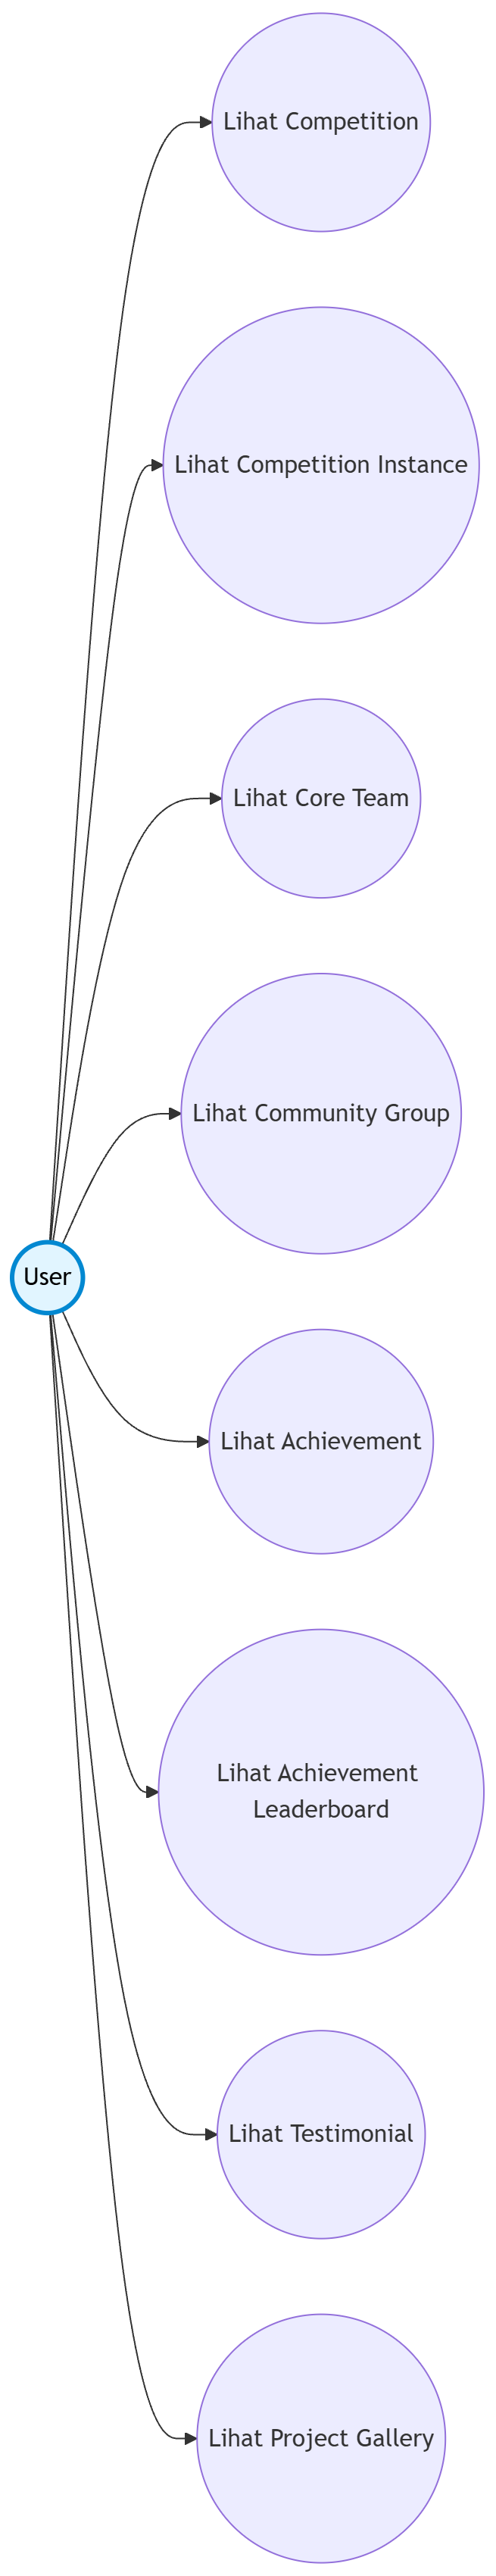
\includegraphics[height=0.8\textheight,keepaspectratio]{images/umls/use-case-public-diagram.png}
                        \end{figure}

                        Pembagian jenis aktor yang ada adalah aktor publik dan aktor terautentikasi. Aktor publik dapat melihat data sistem yang memang diperuntukkan untuk informasi publik, seperti yang terlihat pada \figref{fig:use-case-public-diagram}. Sedangkan aktor terautentikasi dapat mengakses seluruh fitur sistem sesuai dengan hak akses yang dimilikinya untuk menambahkan, mengubah, atau menghapus data sistem, seperti yang dapat dilihat pada \annexref{annex:use-case-diagram-authenticated-user}. Deskripsi mengenai fungsi setiap \textit{use case} dapat dilihat pada \annexref{annex:use-case-description}.

                  \item \textit{Class Diagram}

                        \textit{Class Diagram} merepresentasikan struktur entitas-entitas dalam sistem beserta atribut, metode, dan relasi antar entitas, sebagaimana yang terlihat pada \figref{fig:class-diagram}. Sistem informasi organisasi INFINITE memiliki 35 entitas, yang dapat dikelompokkan ke dalam beberapa domain utama:

                        \begin{figure}
                              \centering
                              \caption{\textit{Class Diagram}}
                              \label{fig:class-diagram}
                              \vspace{-2cm}
                              \makebox[\textwidth][c]{\includegraphics[height=1.06\textwidth,angle=270,keepaspectratio]{images/umls/class-diagram.png}}
                        \end{figure}

                        \begin{itemize}
                              \item Domain Otorisasi: \texttt{Group}, \texttt{Permission}, \texttt{UserGroup}, \texttt{GroupPermission}, \texttt{UserPermission}.
                              \item Domain Pengguna: \texttt{User}, \texttt{Persona}, \texttt{UserPersona}, \texttt{Token}.
                              \item Domain Akademik: \texttt{Degree}, \texttt{Faculty}, \texttt{Major}.
                              \item Domain Organisasi: \texttt{CoreTeam}, \texttt{CoreTeamDivision}, \texttt{CoreTeamMember}, \texttt{CommunityGroup}, \texttt{CommunityGroupAdmin}, \texttt{CommunityGroupMember}, \texttt{CommunityGroupAdminMember}.
                              \item Domain Kompetisi: \texttt{Competition}, \texttt{CompetitionInstance}, \texttt{CompetitionOrganizerType}, \texttt{CompetitionScale}, \texttt{CompetitionRank}, \texttt{CompetitionTimeRange}, \texttt{CompetitionOutput}, \texttt{CompetitionTeamType}.
                              \item Domain Pendanaan dan Prestasi Tim: \texttt{Team}, \texttt{TeamMember},  \texttt{FundApplication}, \texttt{Achievement}, \texttt{AchievementLeaderboard}.
                              \item Domain Konten: \texttt{Testimonial}, \texttt{ProjectGallery}.
                              \item Domain Konfigurasi: \texttt{Config}.
                        \end{itemize}

                        Entitas \texttt{User} memiliki atribut terkomputasi \texttt{is\_active} yang didapatkan dari perbandingan tanggal saat ini dengan tanggal \texttt{end\_date} yang menandai akhir masa aktif anggota. Selain itu, entitas \texttt{Achievement} juga memiliki atribut terkomputasi \texttt{point} yang dihitung dari perkalian bobot enam taksonomi kompetisi (\texttt{organizer\_type $\times$ team\_type $\times$ scale $\times$ time\_range $\times$ output $\times$ rank}), yang selanjutnya diakumulasi ke dalam \texttt{AchievementLeaderboard} per pengguna per tahun.

                  \item \textit{Sequence Diagram}

                        \textit{Sequence Diagram} menggambarkan alur interaksi antar objek dalam sistem berdasarkan urutan waktu. Diagram ini membantu memahami mekanisme kerja dan proses transaksi data yang terjadi dalam sistem. Beberapa \textit{sequence diagram} utama yang dirancang meliputi: alur autentikasi OIDC (mulai dari \textit{redirect} ke SSO hingga pembuatan sesi pengguna), alur pengelolaan keseluruhan data sistem secara umum (\textit{CRUD}), dan alur sinkronisasi data pengguna dan hak akses/otorisasi ke sistem SSO. \textit{Sequence diagram} yang dirancang disajikan pada \figref{fig:sequence-auth-oidc}, \figref{fig:sequence-sso-sync}, dan \figref{fig:sequence-request}.

                        \begin{figure}
                              \centering
                              \caption{\textit{Sequence Diagram} Alur Autentikasi OIDC}
                              \label{fig:sequence-auth-oidc}
                              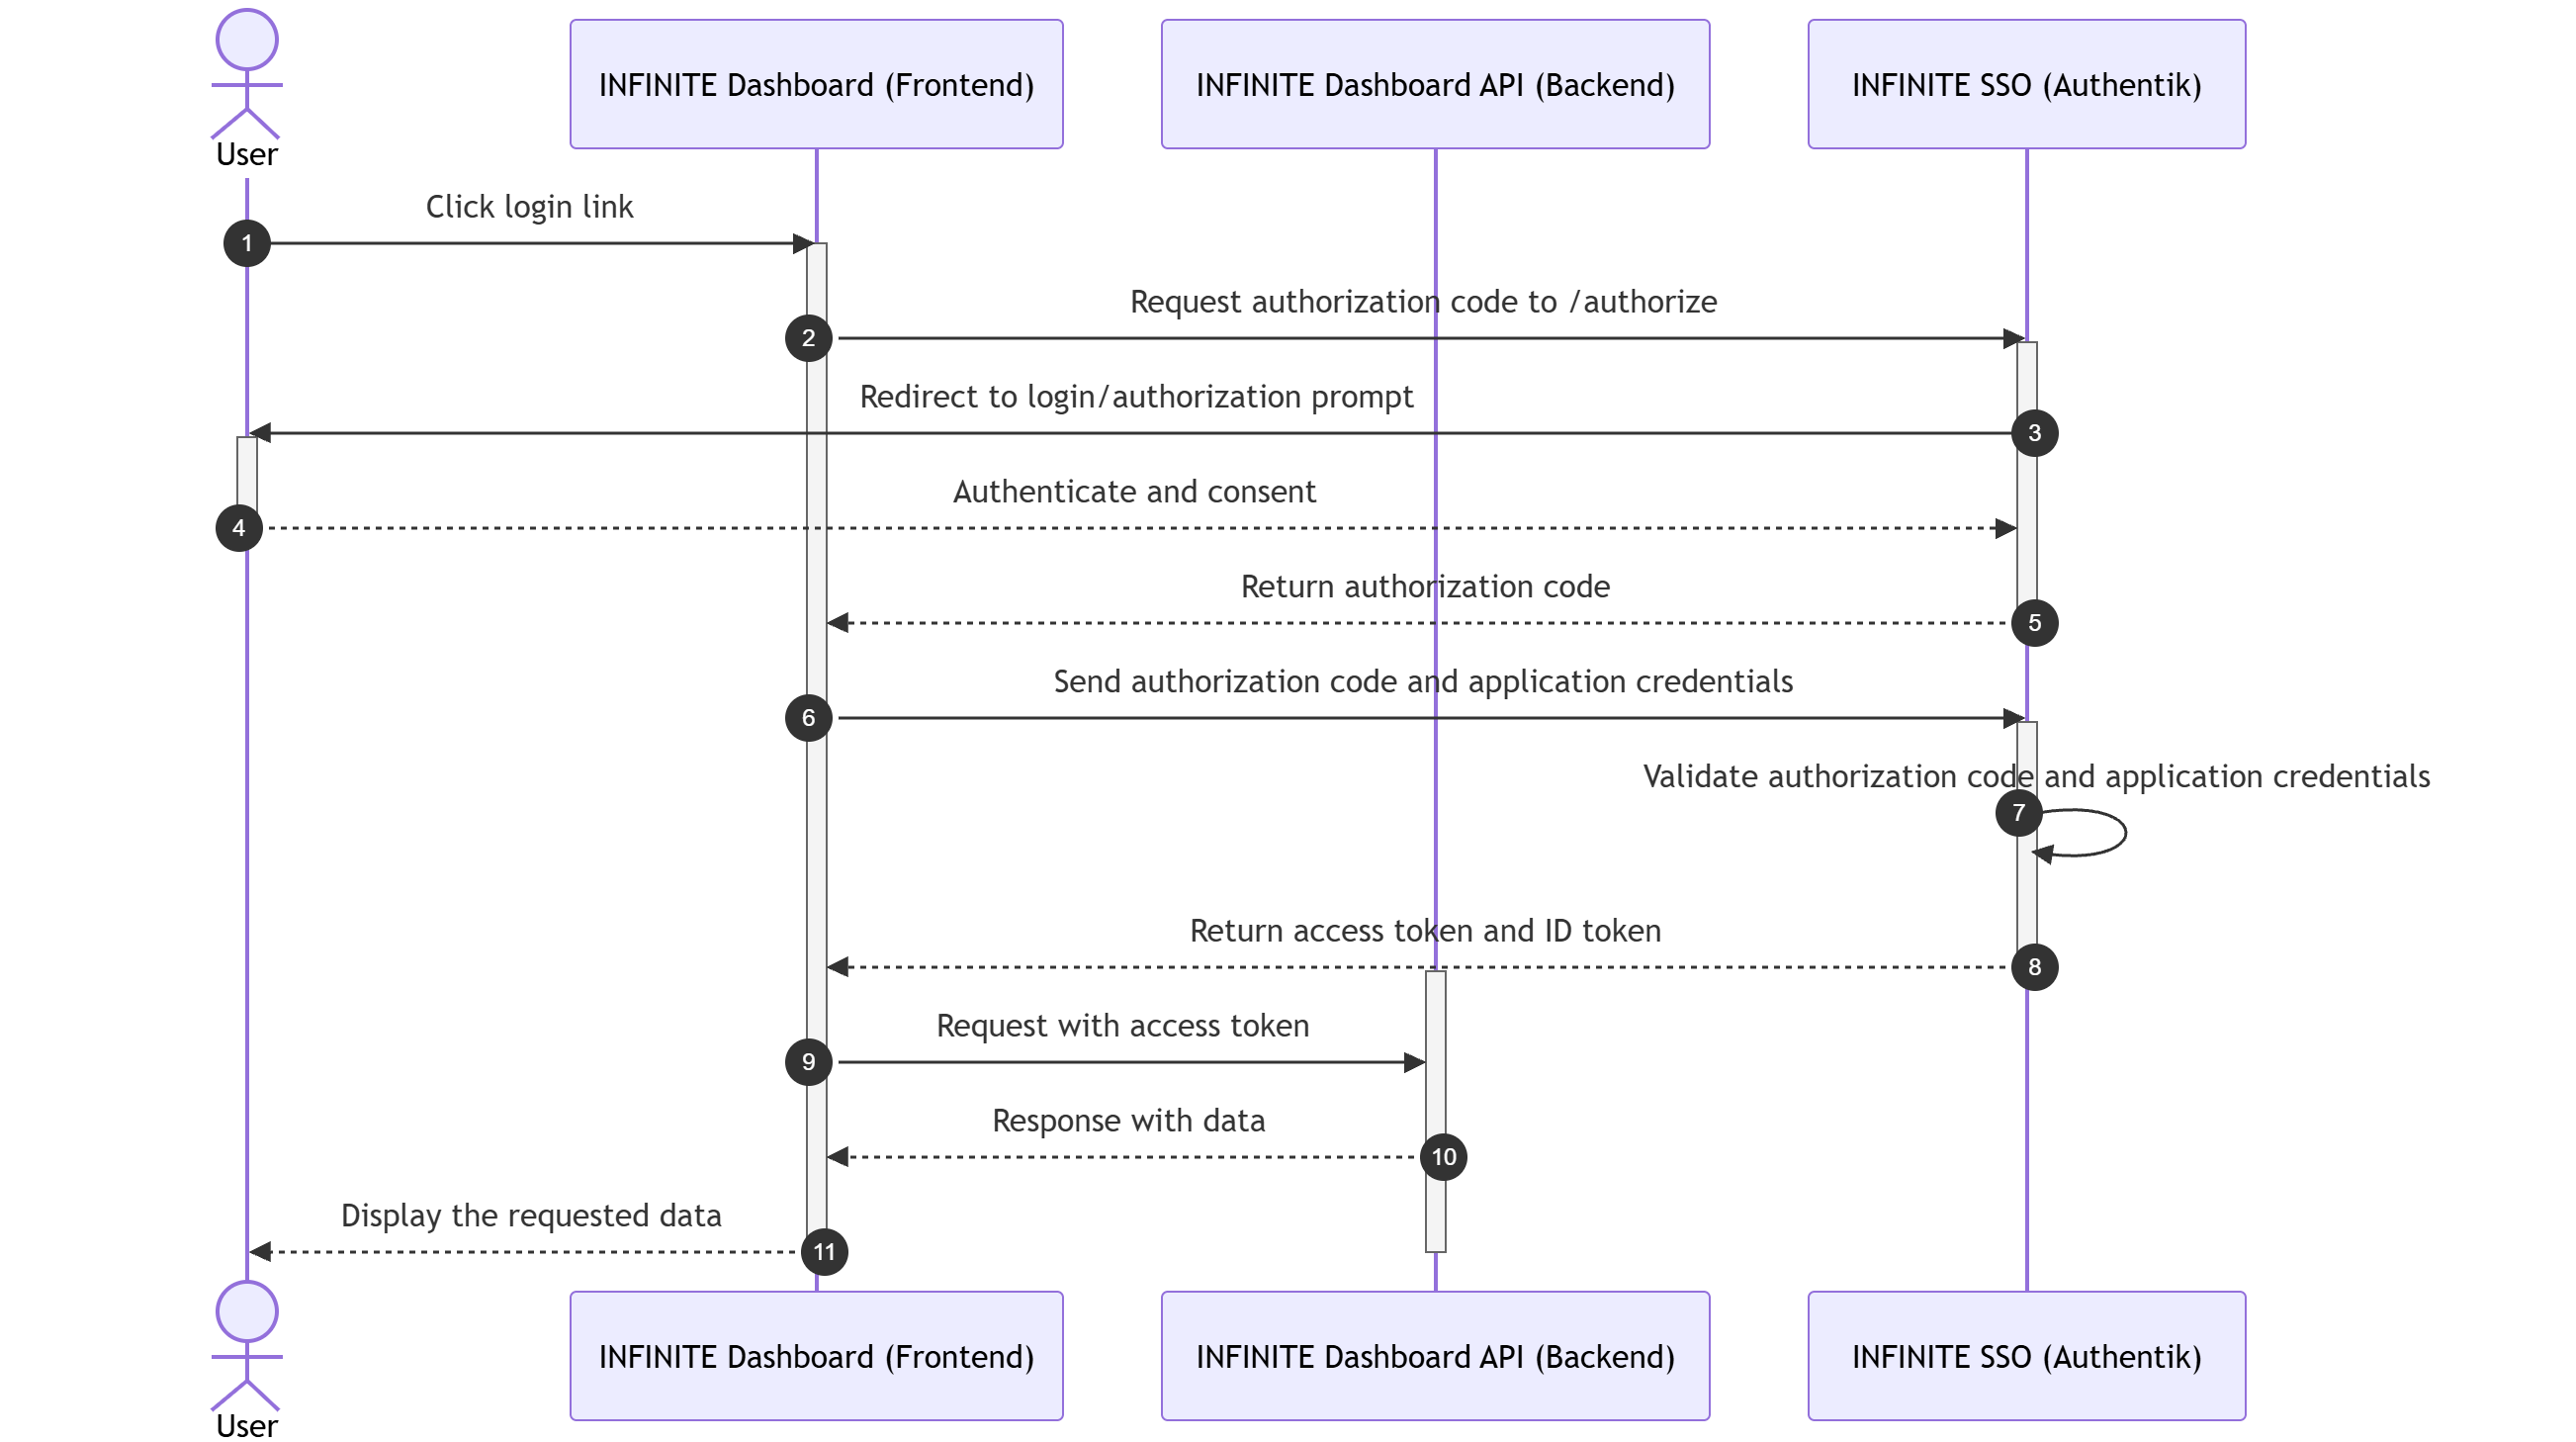
\includegraphics[width=1\textwidth,keepaspectratio]{images/umls/auth-oidc-sequence-diagram.png}
                        \end{figure}

                        \begin{figure}
                              \centering
                              \caption{\textit{Sequence Diagram} Alur Sinkronisasi Data Pengguna dan Hak Akses ke SSO}
                              \label{fig:sequence-sso-sync}
                              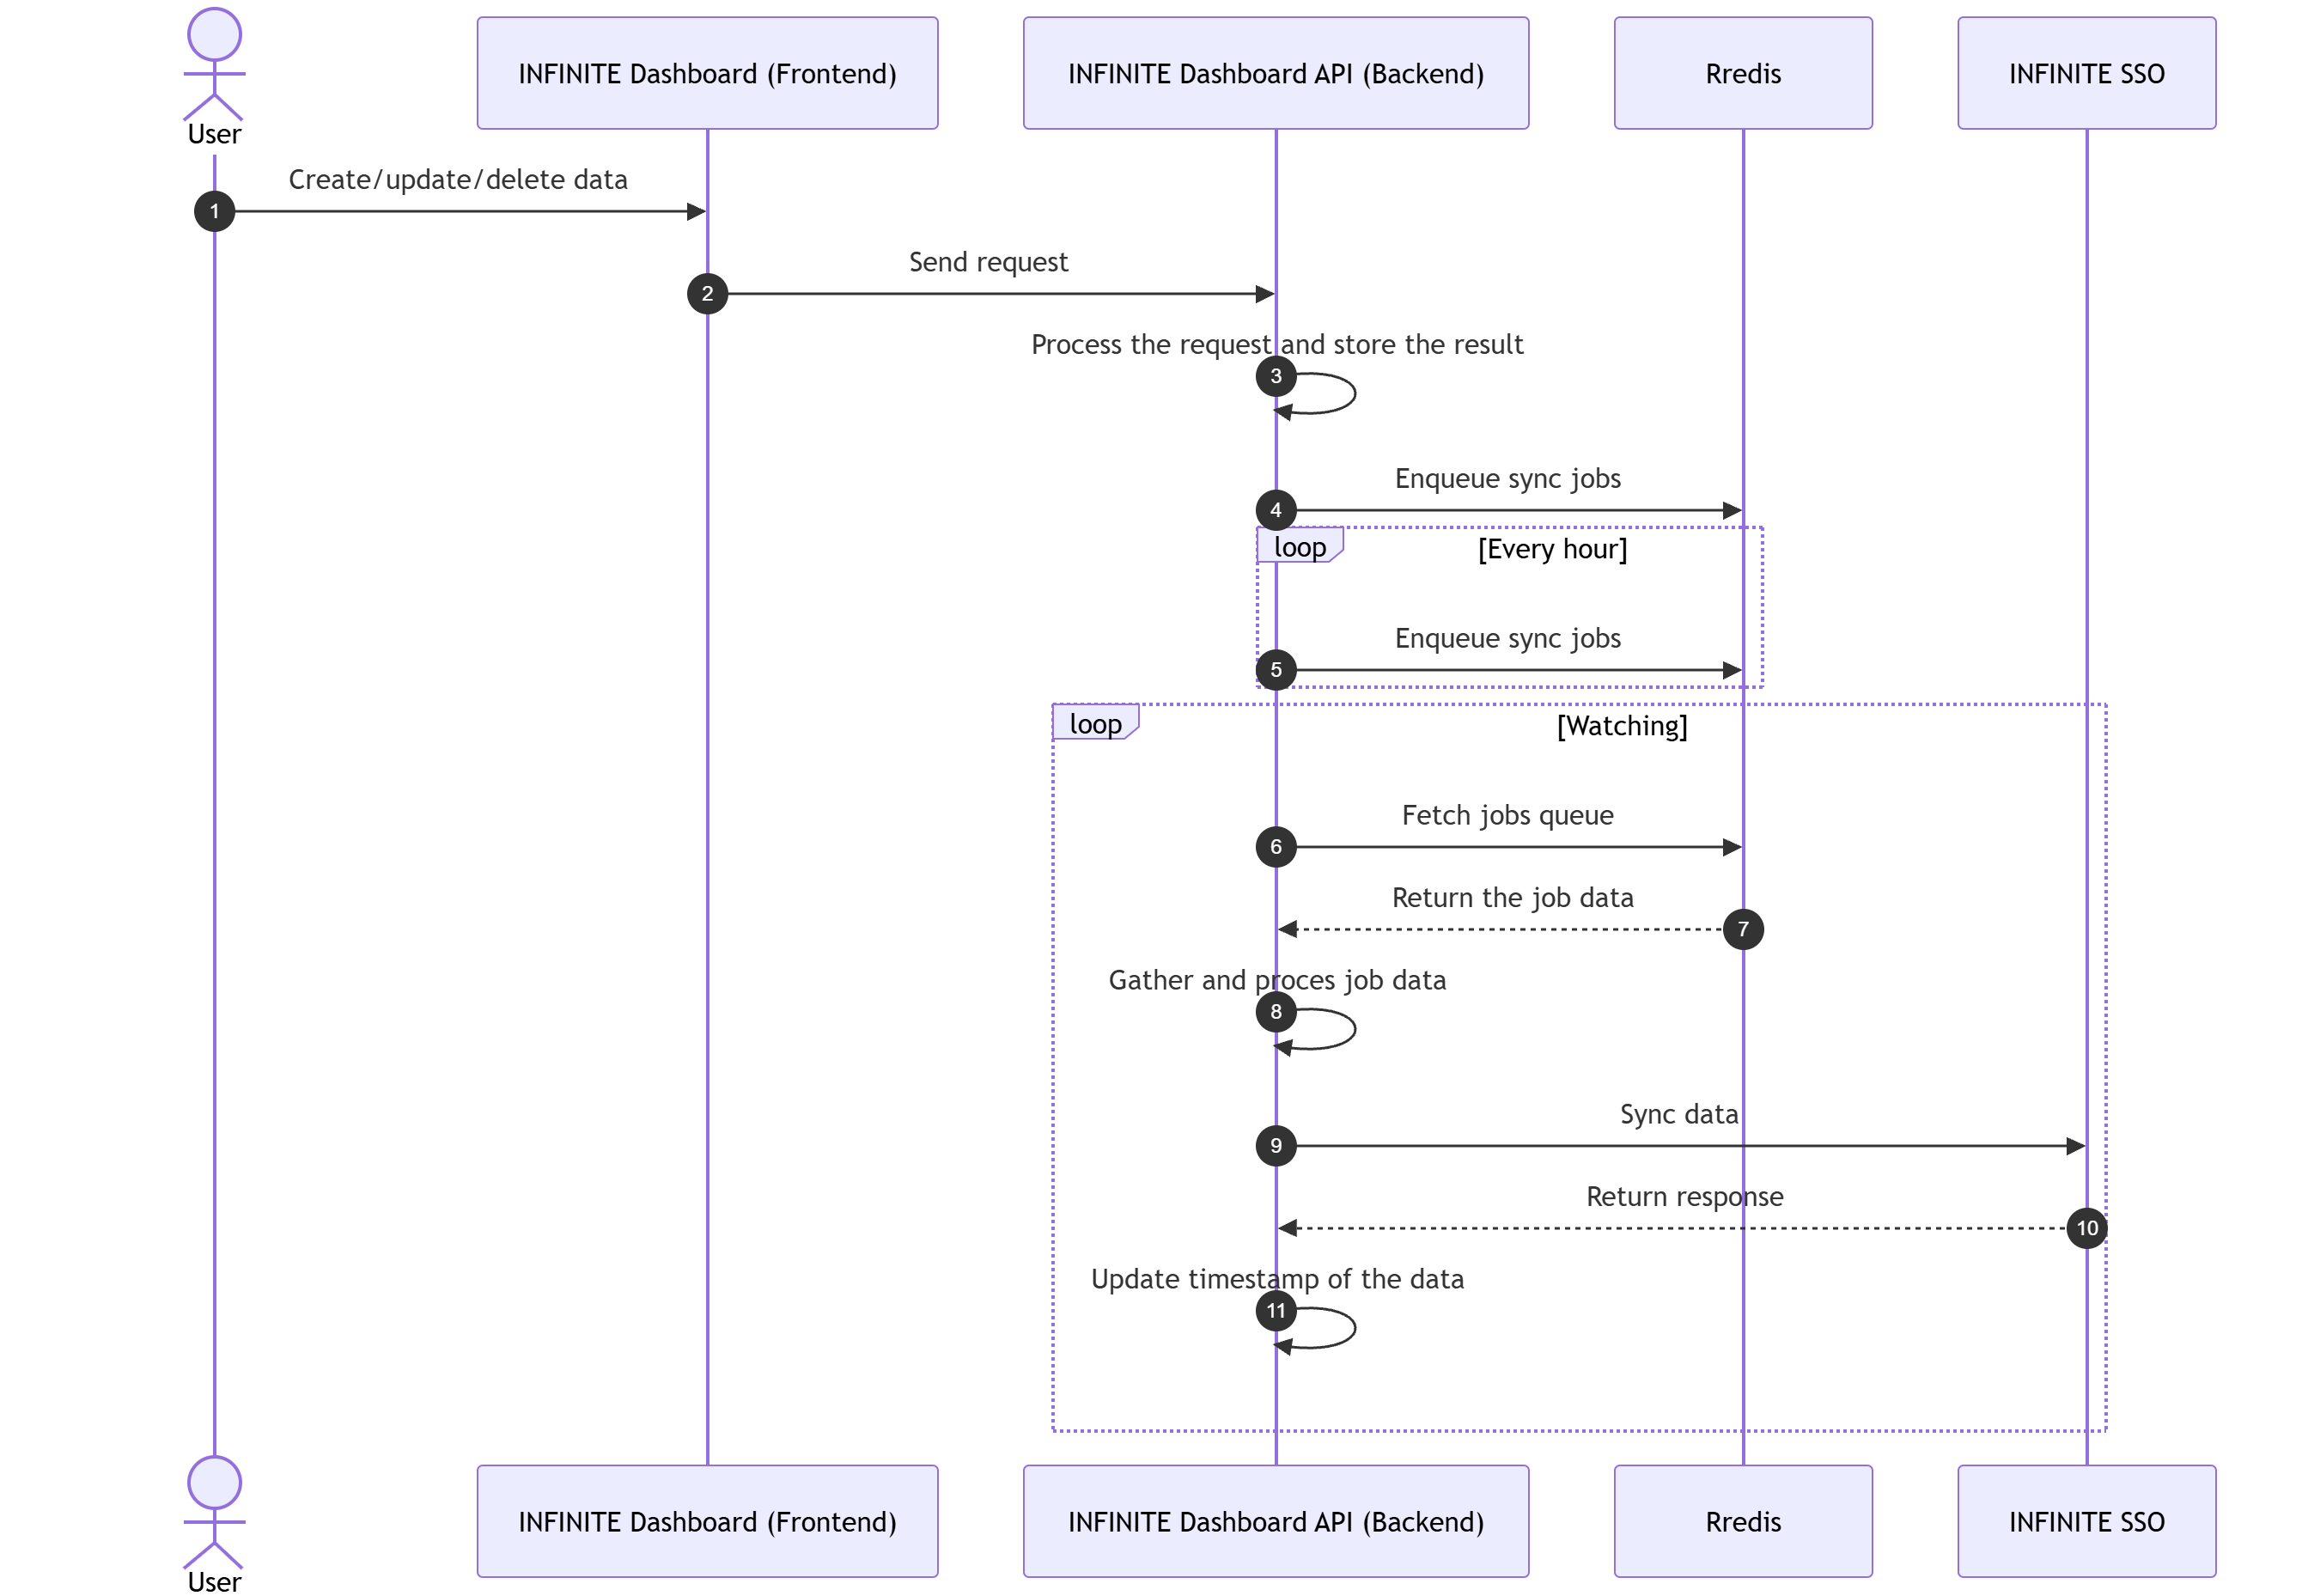
\includegraphics[width=1\textwidth,keepaspectratio]{images/umls/sso-sync-sequence-diagram.png}
                        \end{figure}

                        \begin{figure}
                              \centering
                              \caption{\textit{Sequence Diagram} Alur Pengelolaan Data Sistem (CRUD)}
                              \label{fig:sequence-request}
                              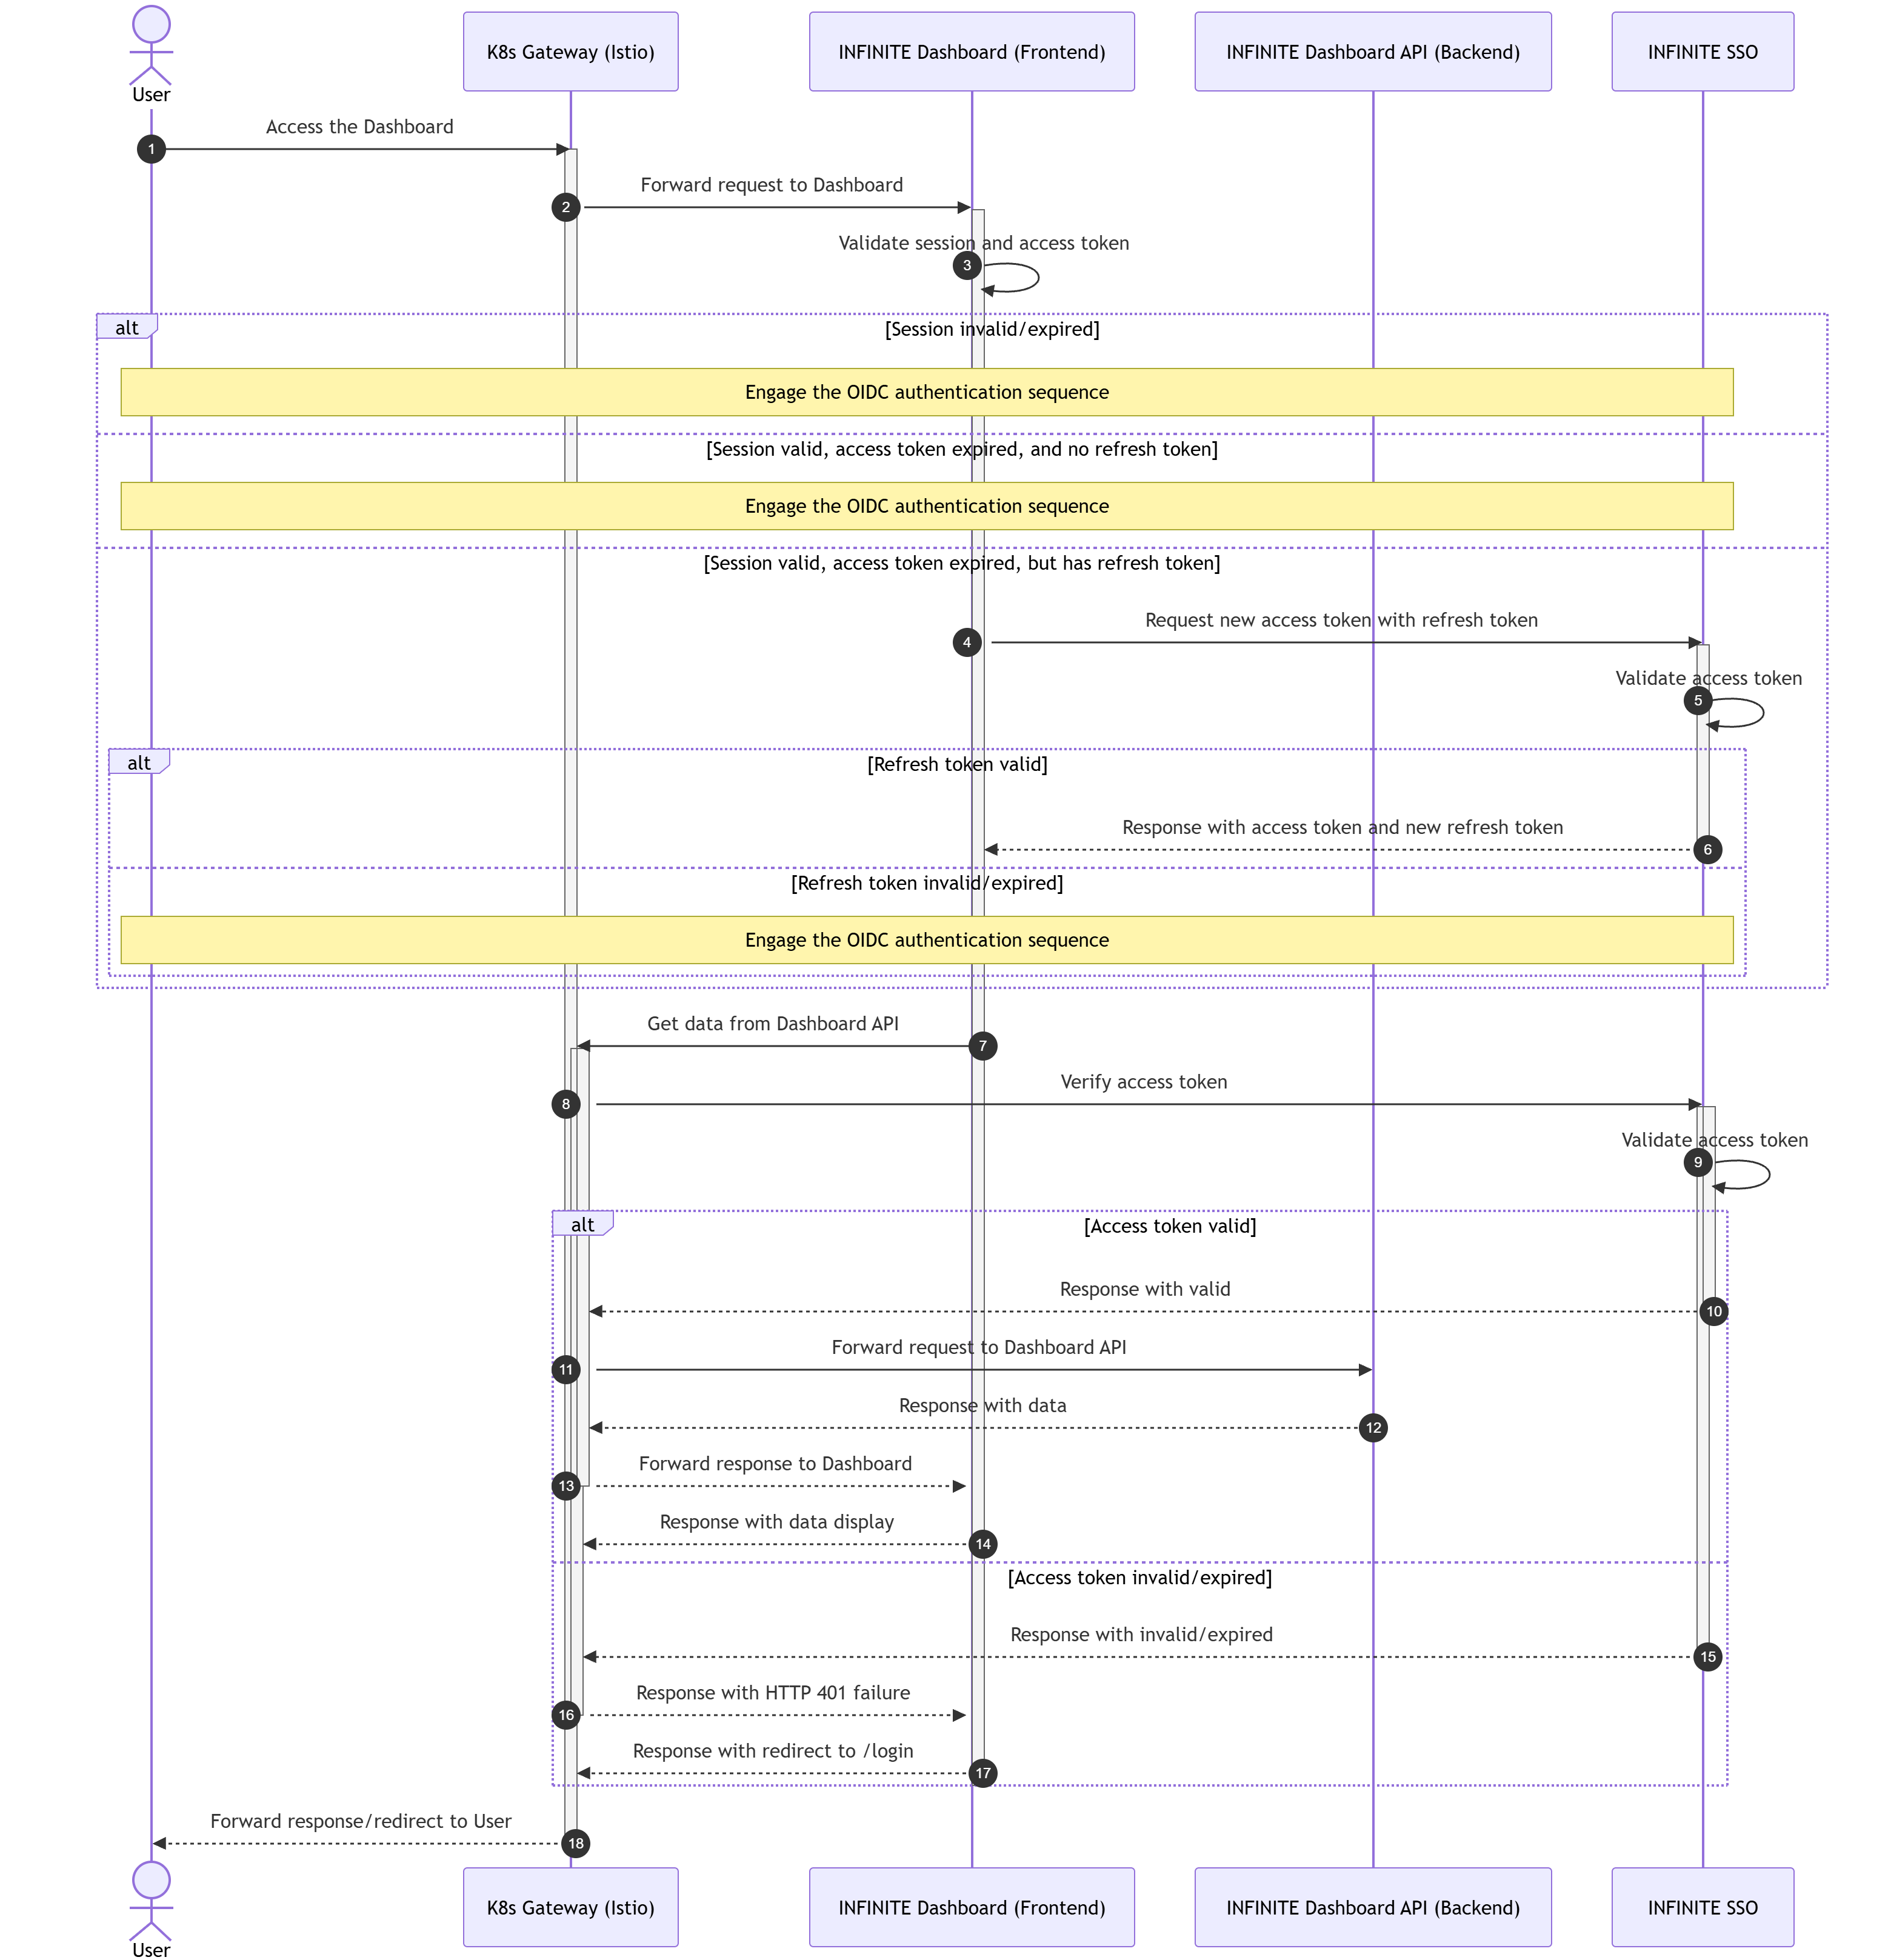
\includegraphics[width=1\textwidth,keepaspectratio]{images/umls/request-sequence-diagram.png}
                        \end{figure}
            \end{enumerate}

      \item Desain Basis Data

            Desain basis data dirancang menggunakan dokumen migrasi dari Laravel dibantu dengan \textit{software} DataGrip untuk menghasilkan 35 tabel basis data. Perancangan basis data mempertimbangkan integritas referensial, efisiensi kueri, dan skalabilitas. Semua tabel menggunakan \textit{primary key} berbasis UUID (\textit{Universally Unique Identifier}) versi 7 untuk menjamin keunikan global dan keamanan namun tetap mendukung pengurutan secara kronologis maupun leksikografis. Relasi antar tabel meliputi relasi satu-ke-banyak (\textit{one-to-many}) seperti \texttt{User} ke \texttt{Achievement}, relasi banyak-ke-banyak (\textit{many-to-many}) seperti \texttt{User} ke \texttt{CoreTeam} melalui \texttt{CoreTeamMember}, serta relasi hierarkis seperti \texttt{Major} ke \texttt{Degree} dan \texttt{Faculty}.

            \begin{figure}[H]
                  \centering
                  \caption{Desain Basis Data}
                  \label{fig:database-design}
                  \makebox[\textwidth][c]{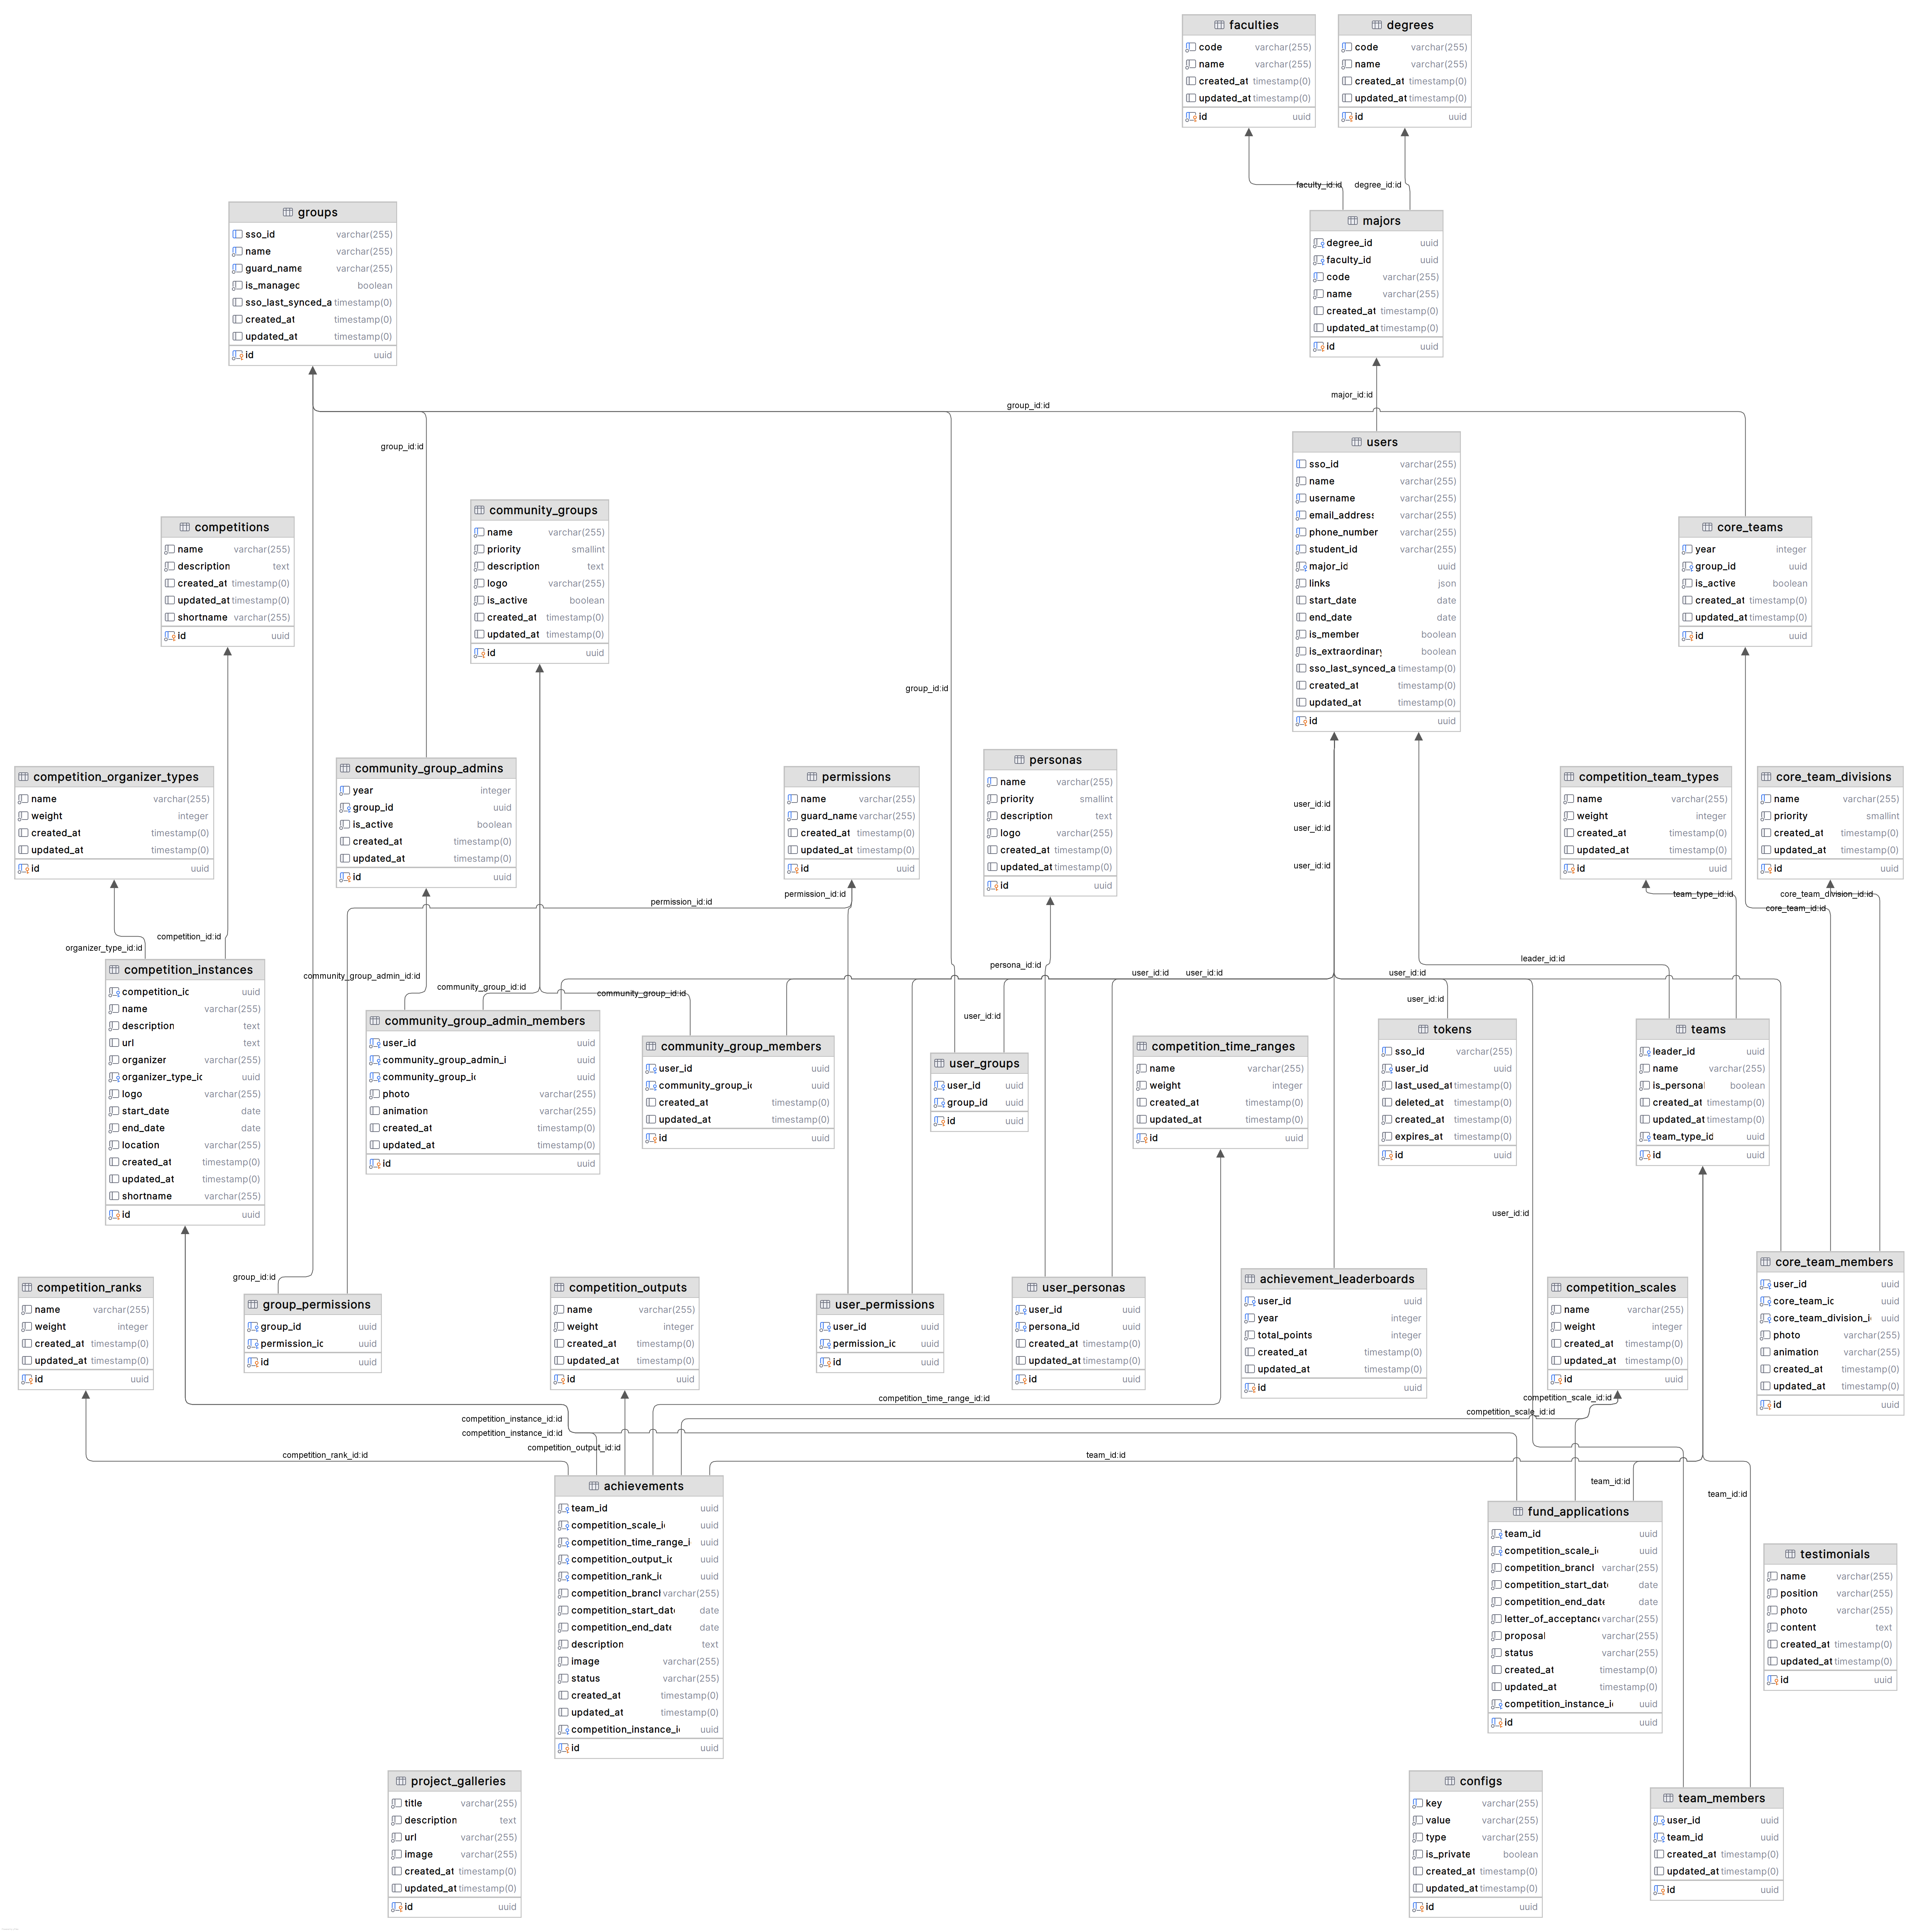
\includegraphics[width=1.34\textwidth,keepaspectratio]{images/entity-relationship-diagram.png}}
            \end{figure}

      \item Desain Antarmuka

            Desain antarmuka \textit{frontend} dirancang menggunakan \textit{software} Figma. Secara garis besar, terdapat 3 jenis desain antarmuka halaman yang dibuat, yaitu halaman list data seperti pada \figref{fig:design-list-page}, halaman detail seperti pada \figref{fig:design-detail-page}, dan halaman formulir sunting seperti pada \figref{fig:design-form-page}. Antarmuka dirancang mengikuti prinsip \textit{responsive design} dengan navigasi berbasis menu atas (\textit{navbar}) dan menu samping (\textit{sidebar}) yang dapat dilipat.

            \begin{figure}[H]
                  \centering
                  \caption{Desain Halaman List Data}
                  \label{fig:design-list-page}
                  \makebox[\textwidth][c]{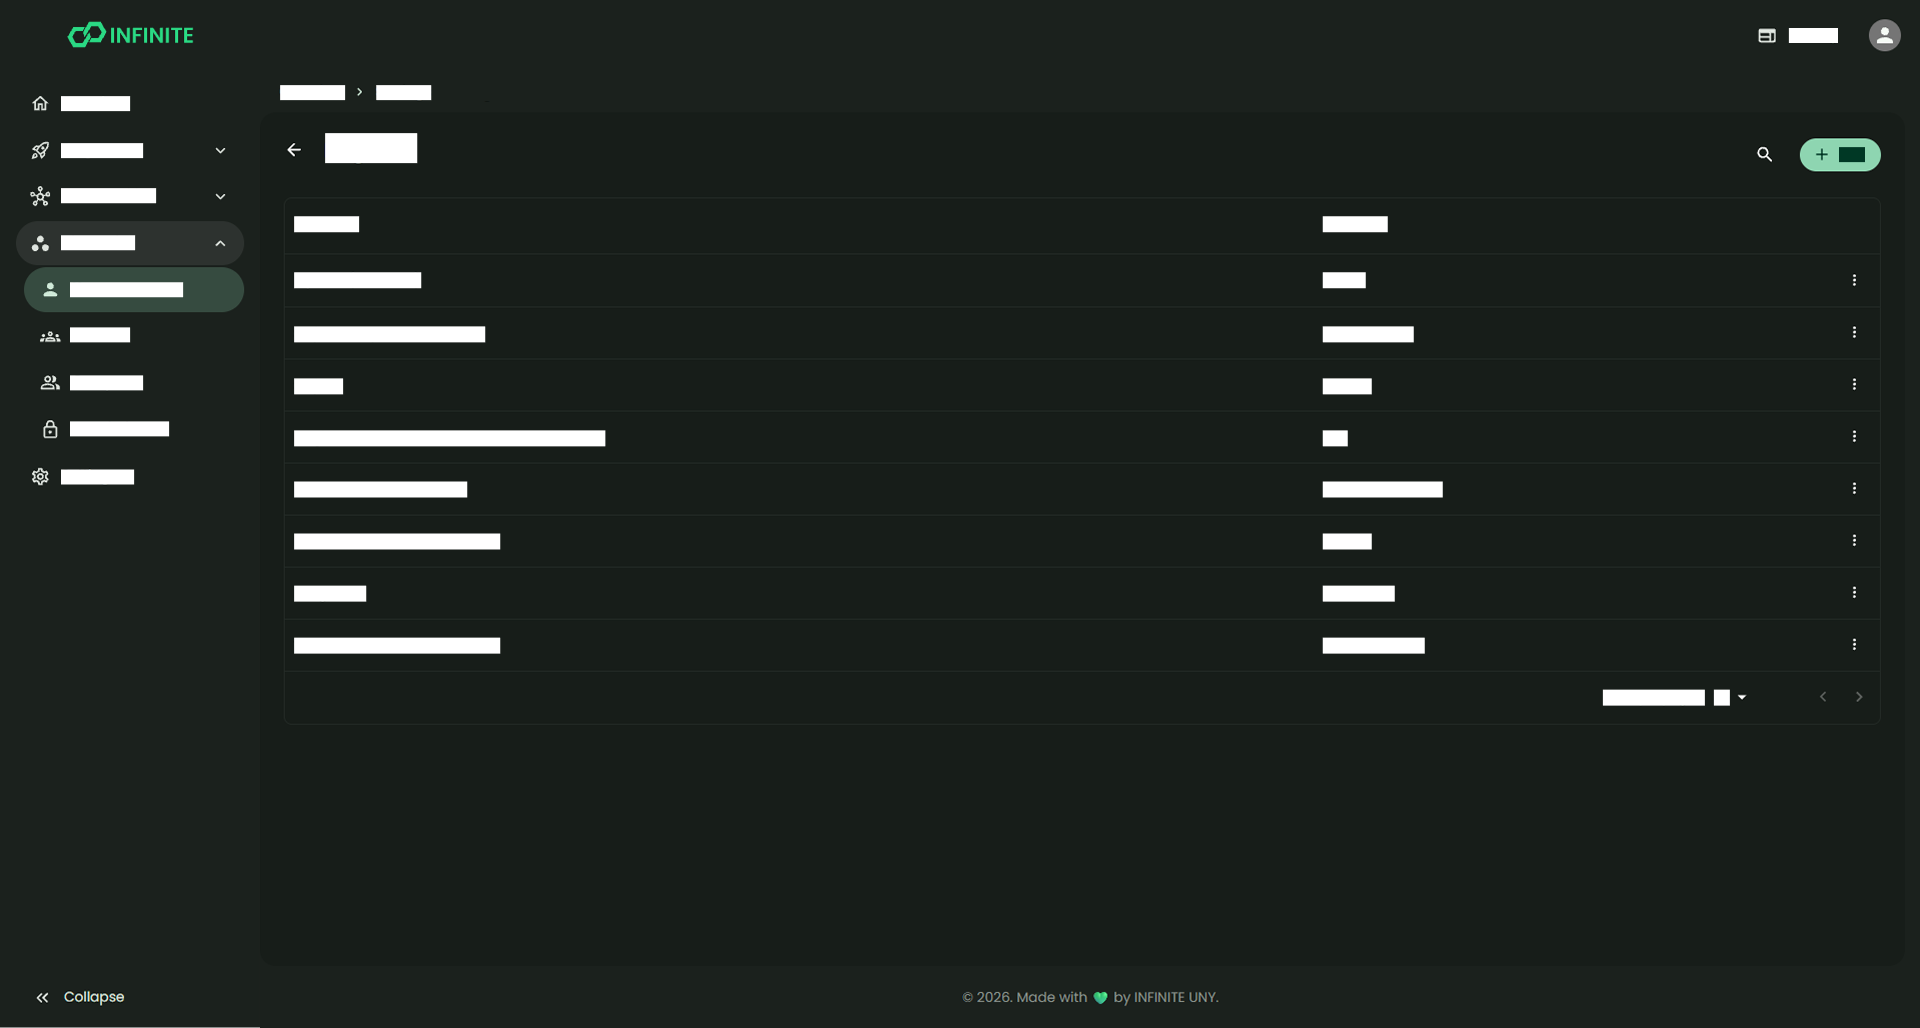
\includegraphics[width=0.9\textwidth,keepaspectratio]{images/design-list-page.png}}
            \end{figure}

            \begin{figure}[H]
                  \centering
                  \caption{Desain Halaman Detail}
                  \label{fig:design-detail-page}
                  \makebox[\textwidth][c]{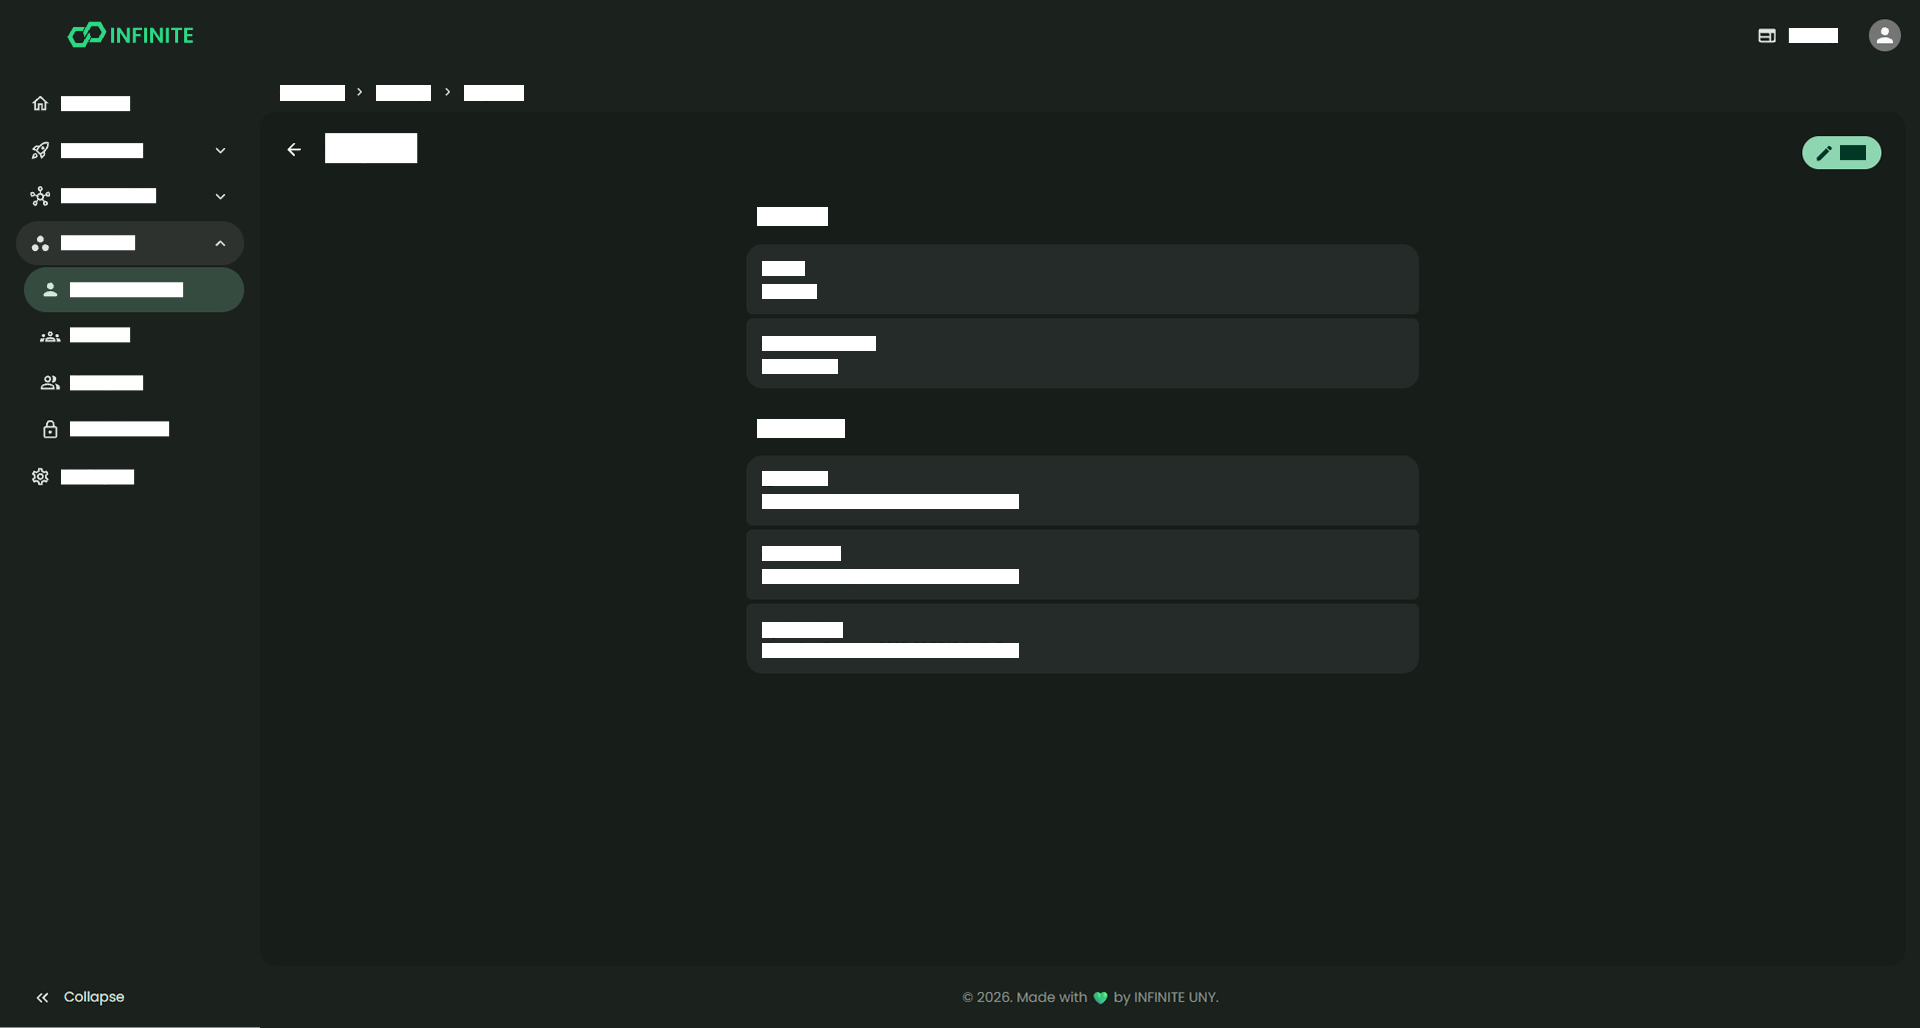
\includegraphics[width=0.9\textwidth,keepaspectratio]{images/design-detail-page.png}}
            \end{figure}

            \begin{figure}[H]
                  \centering
                  \caption{Desain Halaman Formulir Sunting}
                  \label{fig:design-form-page}
                  \makebox[\textwidth][c]{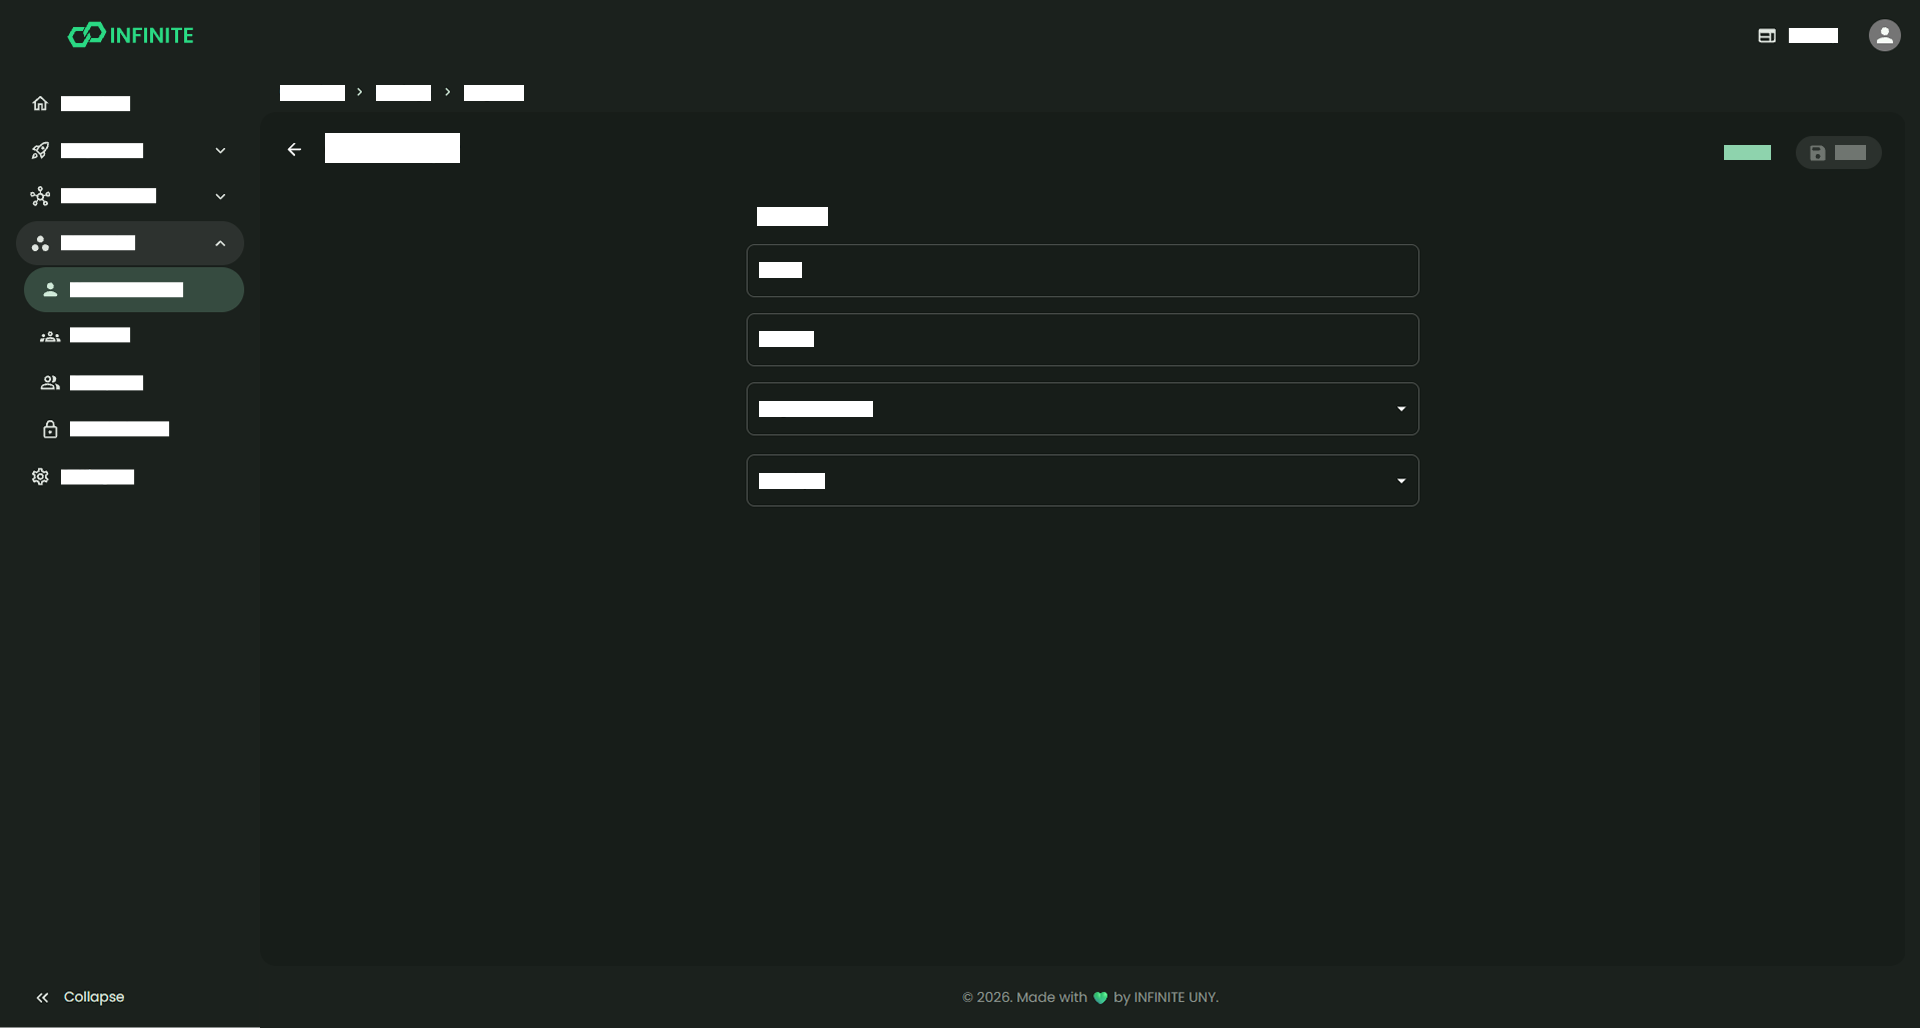
\includegraphics[width=0.9\textwidth,keepaspectratio]{images/design-form-page.png}}
            \end{figure}

\end{enumerate}

\subsubsection{\textit{Implementation and Unit Testing}}

Pada tahap ini, desain yang telah dibuat direalisasikan menjadi kode program yang fungsional. Implementasi dilakukan secara bertahap mulai dari basis data, \textit{backend}, hingga \textit{frontend}.

\begin{enumerate}[listparindent=1cm]
      \item Implementasi Basis Data

            Implementasi basis data dilakukan pada PostgreSQL melalui mekanisme kode program migrasi dari Laravel. Total terdapat 33 berkas kode program migrasi yang mendefinisikan struktur tabel-tabel beserta relasi, indeks, dan \textit{constraint}. Salah satu contoh kode program migrasi untuk tabel \texttt{users} dapat dilihat pada \annexref{annex:code-migration-file}. Setelah berkas migrasi didefinisikan, dilakukan eksekusi migrasi untuk membuat tabel-tabel di basis data PostgreSQL secara otomatis dengan perintah \texttt{php artisan migrate}.

            Selanjutnya, dilakukan implementasi pengisian data awal (\textit{seed}) untuk tabel-tabel referensi seperti data terkait akademik (\texttt{Degree}, \texttt{Faculty}, dan \texttt{Major}), kompetisi (\texttt{CompetitionOrganizerType}, \texttt{CompetitionOutput}, \texttt{CompetitionRank}, \texttt{CompetitionScale}, \texttt{CompetitionTimeRange}, dan \texttt{CompetitionTeamType}), organisasi (\texttt{CoreTeamDivision} dan \texttt{CommunityGroup}), profil pengguna (\texttt{Persona}), serta otorisasi (\texttt{Permission} dan \texttt{Group}) melalui berkas kode program \textit{seeder} Laravel. Salah satu contoh kode program \textit{seeder} untuk data \texttt{groups} dapat dilihat pada \annexref{annex:code-seeder-file}. Eksekusi \textit{seeder} dilakukan dengan perintah \texttt{php artisan db:seed} untuk mengisi data awal ke dalam tabel-tabel basis data yang telah dibuat sebelumnya.

      \item Implementasi \textit{Backend}

            \textit{Backend} sistem informasi organisasi INFINITE dikembangkan menggunakan \textit{framework} Laravel dengan bahasa pemrograman PHP. Arsitektur \textit{backend} mengikuti konsep MVC (\textit{Model-View-Controller}) yang diadaptasi untuk pendekatan \textit{headless}, di mana komponen \textit{View} tidak menghasilkan HTML melainkan respons JSON melalui \textit{API Resources}. Penerapan arsitektur pada \textit{backend} adalah sebagai berikut:

            \begin{enumerate}[listparindent=1cm, label=\alph*.]
                  \item \textbf{\textit{Model}}

                        Sebanyak 35 \textit{model} diimplementasikan untuk merepresentasikan tabel basis data. Akses \textit{query} ke basis data tidak dilakukan secara manual, melainkan melalui Eloquent ORM bawaan Laravel. Setiap \textit{model} menggunakan \textit{trait} \texttt{HasUuids} untuk \textit{primary key} UUID dan menerapkan metode \texttt{serializeDate()} dengan format \texttt{DATE\_ATOM} (ISO 8601) untuk konsistensi serialisasi tanggal. Selain itu, setiap \textit{model} juga mendeklarasikan fungsi relasi antar \textit{model} seperti \texttt{hasMany()}, \texttt{belongsTo()}, dan \texttt{belongsToMany()} untuk mempermudah pemanggilan relasi. Contoh kode program dapat dilihat pada \annexref{annex:code-model-file}

                  \item \textbf{\textit{View}}

                        \textit{View} diimplementasikan menggunakan \textit{API Resource} Laravel yang mengubah \textit{model} menjadi format JSON. Setiap \textit{model} memiliki \textit{resource} dan \textit{resource collection}. Format JSON mengikuti konvensi JSend yang dimodifikasi, dengan struktur \texttt{\{status, data, message\}}. \textit{Resource} dan \textit{resource collection} dibuat secara \textit{custom} dan universal mengikuti format tersebut dengan melakukan ekstensi terhadap \texttt{JsonResource} dan \texttt{ResourceCollection} bawaan Laravel, seperti pada \annexref{annex:code-base-resource-file} dan \annexref{annex:code-base-collection-file}.
                        Setiap \textit{model} kemudian melakukan ekstensi terhadap \textit{custom resource} dan \textit{custom resource collection} tersebut untuk menghasilkan format JSON yang konsisten. Contoh implementasi \textit{resource} dan \textit{resource collection} untuk \textit{model} \texttt{User} dapat dilihat pada \annexref{annex:code-user-resource-file} dan \annexref{annex:code-user-collection-file}.

                  \item \textbf{\textit{Controller}}

                        \textit{Controller} API diorganisasikan dalam direktori \texttt{app/Http/Controllers/Api/V1/} dengan versi API konsisten pada prefix \texttt{/v1/}. Setiap controller menggunakan Spatie \texttt{QueryBuilder} dengan daftar eksplisit untuk kolom yang boleh disertakan (\texttt{allowedIncludes}), disaring (\texttt{allowedFilters}), dan diurutkan (\texttt{allowedSorts}). Seluruh \textit{endpoint} \texttt{index} menggunakan \texttt{cursorPaginate()} untuk paginasi berbasis kursor. Otorisasi diterapkan melalui middleware \texttt{can} dan \texttt{authorizeResource} yang merujuk konfigurasi \textit{policy} untuk setiap \textit{model}. Contoh kode program dapat dilihat pada \annexref{annex:code-user-controller-file}
            \end{enumerate}

            Selain implementasi MVC, \textit{backend} juga mengimplementasikan beberapa pola desain dan mekanisme tambahan untuk mendukung kebutuhan sistem:

            \begin{enumerate}[listparindent=1cm, label=\alph*.]
                  \item \textbf{\textit{Services} dan \textit{Repositories}}

                        Lapisan layanan (\textit{service}) dan repositori (\textit{repository}) diimplementasikan dengan pola \textit{interface-implementation}. \textit{Interface} didefinisikan untuk setiap layanan dan repositori sebagai "kontrak" atau panduan, kemudian \textit{implementation} konkrit diregister sebagai \textit{singleton} di \texttt{AppServiceProvider}. Layanan dan repositori utama meliputi:

                        \begin{itemize}
                              \item \texttt{OidcService}/\texttt{OidcServiceImpl}: menangani verifikasi token JWT OIDC, introspeksi token, dan pengambilan informasi pengguna dari \textit{identity provider}. Kode program dapat dilihat pada \annexref{annex:code-oidc-service-file}
                              \item \texttt{SsoService}/\texttt{SsoServiceImpl}: menangani operasi CRUD terhadap API Authentik SSO untuk sinkronisasi pengguna dan otorisasi. Kode program dapat dilihat pada \annexref{annex:code-sso-service-file}
                              \item \texttt{StorageRepository}/\texttt{StorageRepositoryImpl}: abstraksi penyimpanan berkas dengan pelacakan manifest JSON. Berkas lama dihapus secara asinkron melalui \textit{job} \texttt{DeleteBlob}. Kode program dapat dilihat pada \annexref{annex:code-storage-repository-file}
                        \end{itemize}

                  \item \textbf{Autentikasi \textit{Custom}}

                        Sistem autentikasi \textit{backend} mengimplementasikan tiga \textit{guard} \textit{custom}:

                        \begin{itemize}
                              \item \texttt{OidcTokenGuard}: autentikasi berbasis token Bearer yang memverifikasi tanda tangan JWT melalui OIDC, mencari pengguna berdasarkan \texttt{sso\_id} dengan \textit{fallback} ke pencocokan email, serta melacak token di basis data. Kode program dapat dilihat pada \annexref{annex:code-oidc-token-guard-file}
                              \item \texttt{OidcHeadersGuard}: autentikasi berbasis header untuk mandukung konfigurasi \textit{reverse proxy} yang menangani OIDC di lapisan \textit{proxy}. Kode program dapat dilihat pada \annexref{annex:code-oidc-headers-guard-file}
                              \item \texttt{DummyGuard}: \textit{guard} khusus pengembangan/pengujian yang mengautentikasi sebagai pengguna \textit{dummy}.
                        \end{itemize}

                  \item \textbf{\textit{Job} Asinkron}

                        Sebanyak 20 \textit{job} asinkron dengan antrean diimplementasikan untuk kalkulasi poin prestasi, penghapusan berkas lama, serta menjaga sinkronisasi data antara sistem \textit{backend} dan sistem SSO INFINTE, meliputi pembuatan, pembaruan, dan penghapusan pengguna SSO; sinkronisasi massal pengguna; sinkronisasi keanggotaan grup, pengurus, dan administrator. Antrean didukung oleh Redis Sentinel untuk ketersediaan tinggi. Contoh kode program dapat dilihat pada \annexref{annex:code-sync-achievement-leaderboard-job-file}

                  \item \textbf{Penyimpanan Berkas dengan \textit{Object Storage}}

                        Penyimpanan berkas memanfaatkan \textit{object storage} untuk menyimpan berkas secara efisien dan skalabel. Informasi berkas disimpan dalam manifest JSON yang menyimpan informasi disk, visibilitas, jalur, dan nama berkas ke dalam kolom basis data. \textit{Cast} \texttt{Blob} mengubah manifest menjadi URL saat pembacaan. Berkas privat akan menghasilkan \textit{signed URL} dengan masa berlaku terbatas. Kode program \textit{cast} dapat dilihat pada \annexref{annex:code-model-file}
            \end{enumerate}

      \item Implementasi \textit{Frontend}

            \textit{Frontend} sistem informasi organisasi INFINITE dikembangkan menggunakan Next.js 16 dengan \textit{App Router} dan TypeScript. Arsitektur \textit{frontend} menerapkan prinsip \textit{Clean Architecture} dengan empat lapisan utama yang dipisahkan secara tegas:

            \begin{enumerate}[listparindent=1cm, label=\alph*.]
                  \item \textbf{\textit{Domain}}

                        Merupakan lapisan paling dalam yang berisi aturan bisnis inti tanpa dependensi ke \textit{framework} eksternal. Lapisan ini terdiri dari:

                        \begin{itemize}
                              \item Entitas sebanyak 39 kelas yang merepresentasikan objek bisnis seperti \texttt{User}, \texttt{Team}, \texttt{Achievement}, \texttt{Competition}, \texttt{CoreTeam}, \texttt{FundApplication}, dan lainnya. Contoh kode program dapat dilihat pada \annexref{annex:code-user-entity-file}
                              \item Antarmuka repositori sebanyak 37 berkas yang mendefinisikan kontrak operasi CRUD untuk setiap entitas. Contoh kode program dapat dilihat pada \annexref{annex:code-user-repository-file}
                              \item Kelas kesalahan HTTP dengan kelas dasar \texttt{HttpError} dan turunan seperti \texttt{BadRequestError}, \texttt{UnauthorizedError}, \texttt{ForbiddenError}, \texttt{NotFoundError}, \texttt{ValidationError}, dan \texttt{InternalServerError}. Contoh kode program dapat dilihat pada \annexref{annex:code-http-error-file}
                        \end{itemize}

                  \item \textbf{\textit{Application}}

                        Berisi \textit{use case} sebanyak 165 berkas, masing-masing merupakan kelas \texttt{@injectable()} dengan metode \texttt{execute()}. Setiap \textit{use case} hanya bergantung pada antarmuka repositori di lapisan \textit{domain}. Sebagian besar \textit{use case} yang memerlukan autentikasi terlebih dahulu memanggil \texttt{AuthRepository.getAccessToken()} sebelum meneruskan token ke repositori yang sesuai. Contoh kode program dapat dilihat pada \annexref{annex:code-get-users-usecase-file}

                  \item \textbf{\textit{Infrastructure}}

                        Berisi implementasi konkret dari antarmuka yang didefinisikan di lapisan \textit{domain}:

                        \begin{itemize}
                              \item \textit{Data sources} berupa klien Axios untuk komunikasi API \textit{backend}, konfigurasi autentikasi server dan klien dengan better-auth, serta penyimpanan sesi dan lokal. Contoh kode program dapat dilihat pada \annexref{annex:code-infinity-api-datasource-file}
                              \item \textit{Data Transfer Object} (DTO) dan \textit{mapper} sebanyak 37 berkas yang menyediakan konversi dua arah antara format \textit{snake\_case} API dan format \textit{camelCase} \textit{domain} menggunakan Luxon untuk penanganan tanggal. Contoh kode program dapat dilihat pada \annexref{annex:code-user-dto-file}
                              \item Implementasi repositori sebanyak 37 berkas yang menerima \texttt{InfinityApiDataSource} melalui injeksi dependensi dan melakukan pemanggilan REST API, memetakan kueri untuk penyaringan, pengurutan, dan paginasi berbasis kursor, serta membungkus kesalahan dengan \texttt{handleAxiosError()}. Setiap operasi repositori mengembalikan \texttt{Effect.Either<T, Error>} untuk penanganan kesalahan. Contoh kode program dapat dilihat pada \annexref{annex:code-user-repository-impl-file}
                        \end{itemize}

                  \item \textbf{\textit{Presentation}}

                        Berisi komponen untuk antarmuka pengguna yang diorganisasikan ke dalam:

                        \begin{itemize}
                              \item \textit{Components} yang teridisi dari komponen bersama, komponen autentikasi berisi formulir login dan komponen bersama terkait halaman autentikasi, serta komponen internal berisi 72 direktori komponen untuk setiap entitas, terdiri dari tampilan daftar, tampilan detail, formulir, dan bilah alat. Komponen bersama meliputi \texttt{Header}, \texttt{Footer}, \texttt{Sidebar}, \texttt{Navbar}, \texttt{AlertDialog}, \texttt{PDFViewer}, operator \texttt{DataGrid}, dan lainnya.
                              \item \textit{Controllers} yang berisi \texttt{AuthController} untuk menjembatani better-auth ke \textit{route handlers} Next.js.
                              \item \textit{Hooks} yang berisi \texttt{useInternalStore} sebagai \textit{hook} Zustand untuk menyediakan \textit{state} internal sebagai konteks React.
                              \item \textit{Stores} yang berisi manajemen \textit{state} Zustand dengan \textit{middleware} Immer untuk pembaruan \textit{immutable}.
                        \end{itemize}
            \end{enumerate}

            \begin{figure}
                  \centering
                  \caption{Tampilan Halaman List Data}
                  \label{fig:view-list-page}
                  \makebox[\textwidth][c]{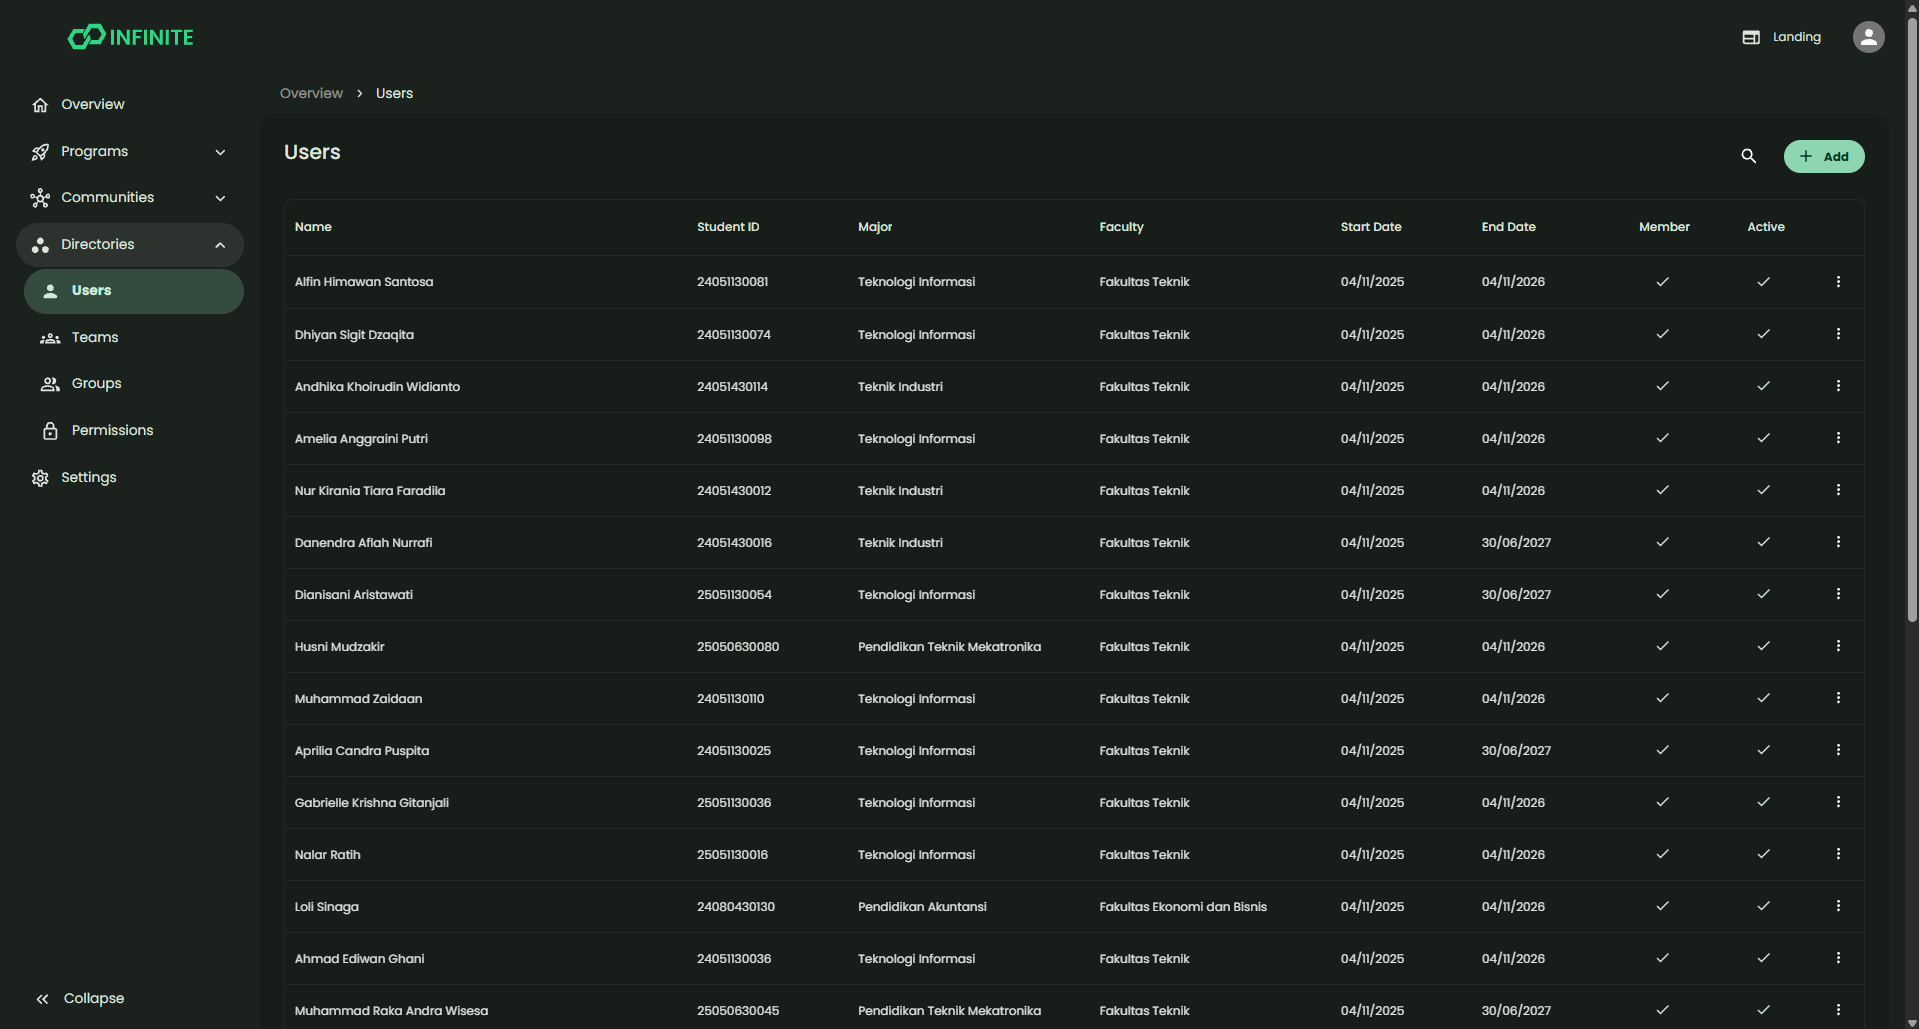
\includegraphics[width=0.9\textwidth,keepaspectratio]{images/tampilan-halaman-list.png}}
            \end{figure}

            \begin{figure}
                  \centering
                  \caption{Tampilan Halaman Detail}
                  \label{fig:view-detail-page}
                  \makebox[\textwidth][c]{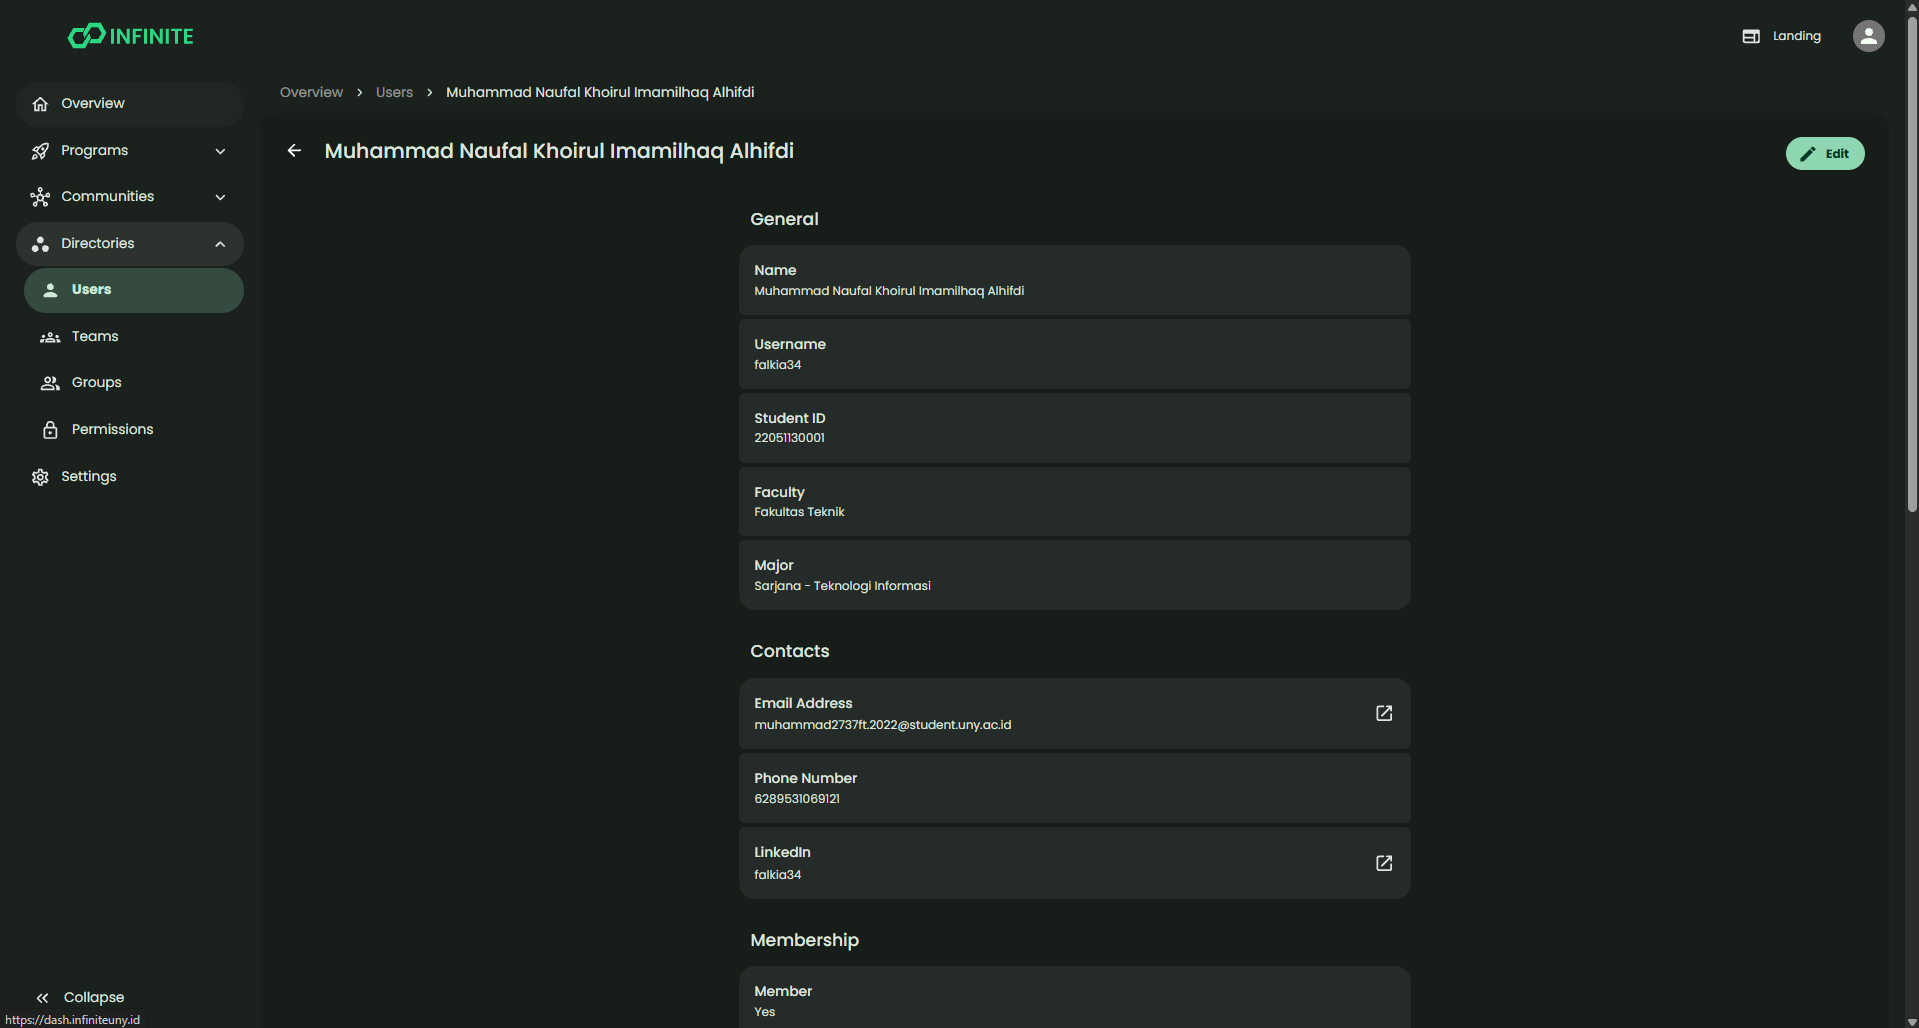
\includegraphics[width=0.9\textwidth,keepaspectratio]{images/tampilan-halaman-detail.png}}
            \end{figure}

            \begin{figure}
                  \centering
                  \caption{Tampilan Halaman Formulir Sunting}
                  \label{fig:view-form-page}
                  \makebox[\textwidth][c]{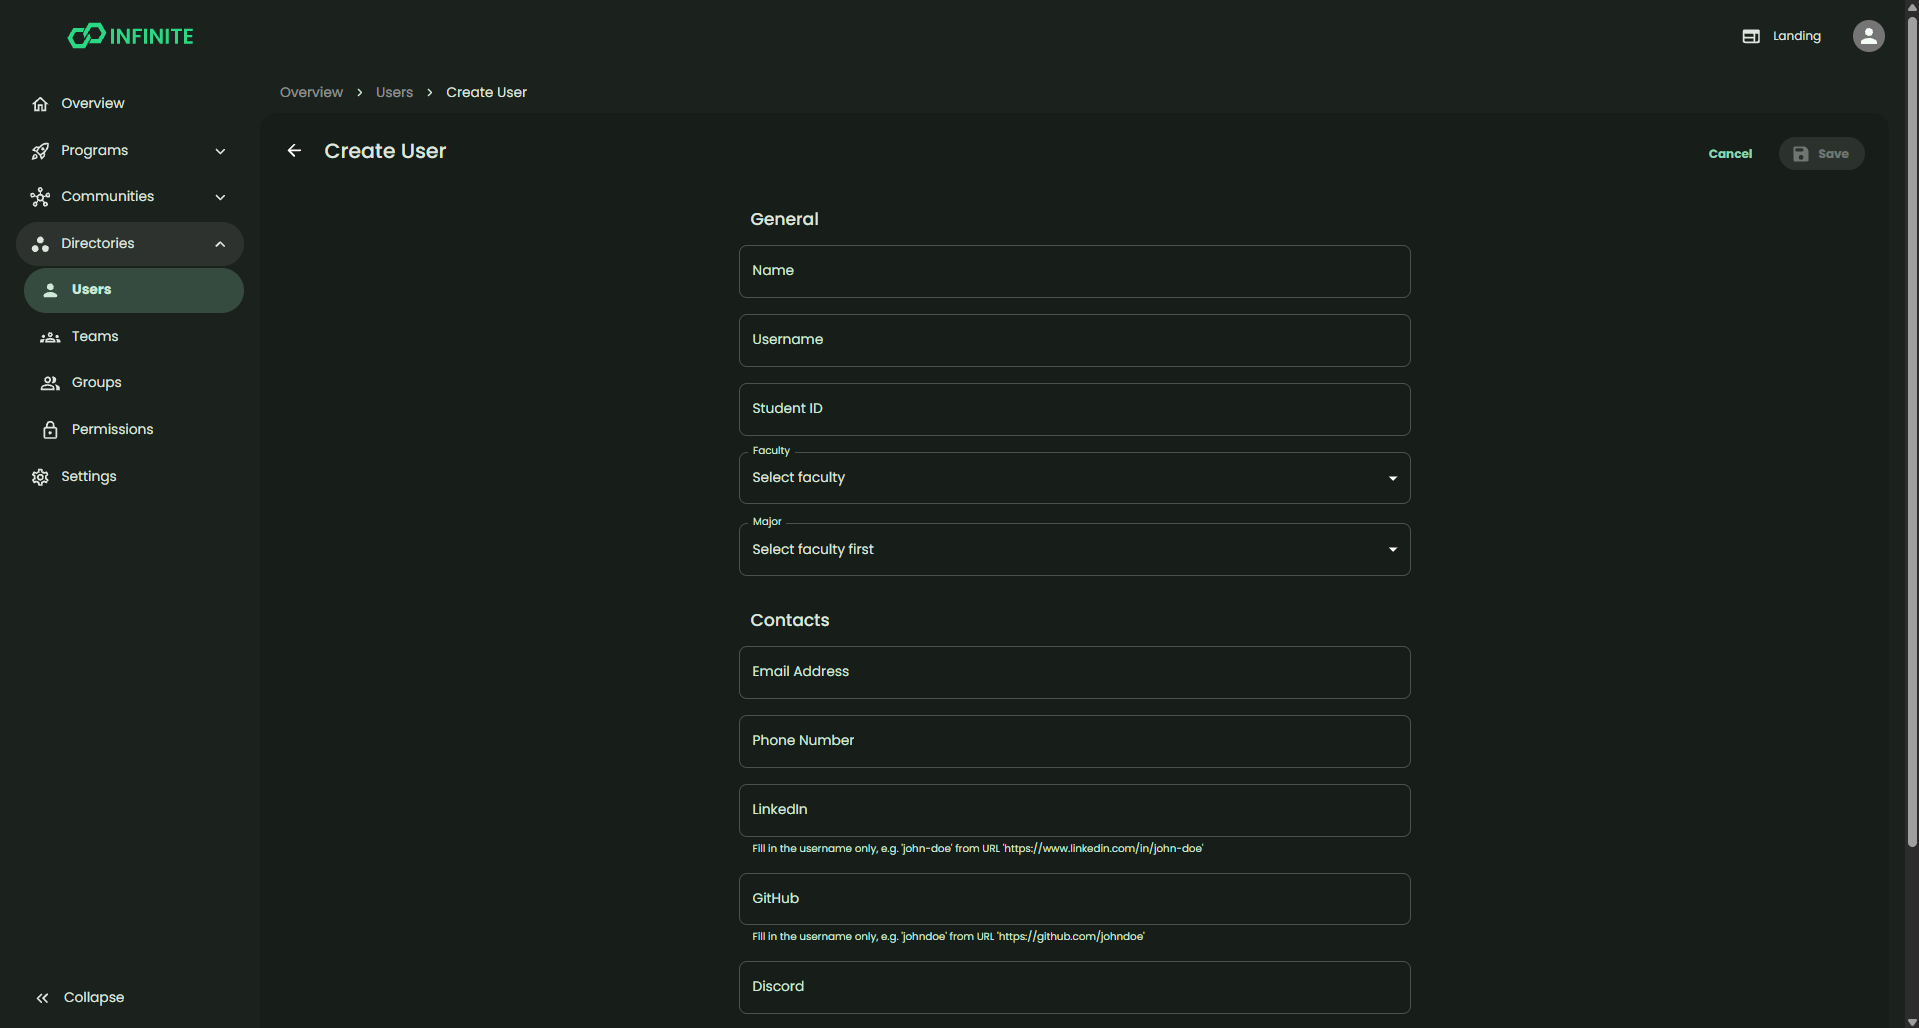
\includegraphics[width=0.9\textwidth,keepaspectratio]{images/tampilan-halaman-form.png}}
            \end{figure}

            Injeksi dependensi diimplementasikan menggunakan Inversify v8 dengan dekorator \texttt{@injectable()} dan injeksi konstruktor \texttt{@inject(SYMBOLS.Xxx)}. Terdapat 215 simbol yang didefinisikan di \texttt{config/symbols.ts} untuk injeksi dependensi. Dibuat juga 2 kontainer untuk melakukan \textit{binding} dependensi, yaitu \texttt{src/server-injection.ts} untuk sisi server (menggunakan \texttt{AuthServerDataSource} dan \texttt{InfinityApiDataSource}), serta \texttt{src/client-injection.ts} untuk sisi klien (menggunakan \texttt{AuthClientDataSource}, \texttt{InfinityApiDataSource}, dan \texttt{SessionStorageDataSource}).

            Konfigurasi \textit{routing} Next.js membagi rute ke dalam tiga grup: \texttt{(auth)} untuk alur autentikasi, \texttt{(internal)} untuk dasbor internal yang terautentikasi, dan \texttt{(public)} untuk rute publik seperti pemeriksaan kesehatan sistem. Konfigurasi \texttt{proxy.ts} dari Next.js diatur untuk memeriksa sesi pada setiap permintaan dan mengarahkan pengguna yang belum terautentikasi ke halaman masuk.

            Autentikasi \textit{frontend} menggunakan \textit{library} better-auth v1.6 dengan plugin \texttt{genericOAuth} untuk integrasi dengan SSO INFINITE berbasis protokol OIDC. Sesi disimpan di Redis Sentinel untuk ketersediaan tinggi, dengan masa berlaku sesi 2 jam yang diperbarui setiap 10 menit. Plugin sesi kustom menambahkan \texttt{internalId}, \texttt{username}, dan \texttt{permissions} ke objek sesi pengguna untuk keperluan kontrol akses di antarmuka.
\end{enumerate}

\subsubsection{\textit{Integration and System Testing}}

Setelah seluruh komponen \textit{backend} dan \textit{frontend} diimplementasikan, dilakukan integrasi sistem dan pengujian kualitas secara menyeluruh.

\begin{enumerate}[listparindent=1cm]
      \item Integrasi Sistem dengan Kubernetes Berbasis GitOps

            Sistem informasi organisasi INFINITE diintegrasikan dan di-\textit{deploy} sebagai aplikasi terkontainerisasi di platform Kubernetes. Proses integrasi mencakup:

            \begin{figure}
                  \centering
                  \caption{CI/CD dengan GitHub Actions dan ArgoCD}
                  \label{fig:pipeline-cicd}
                  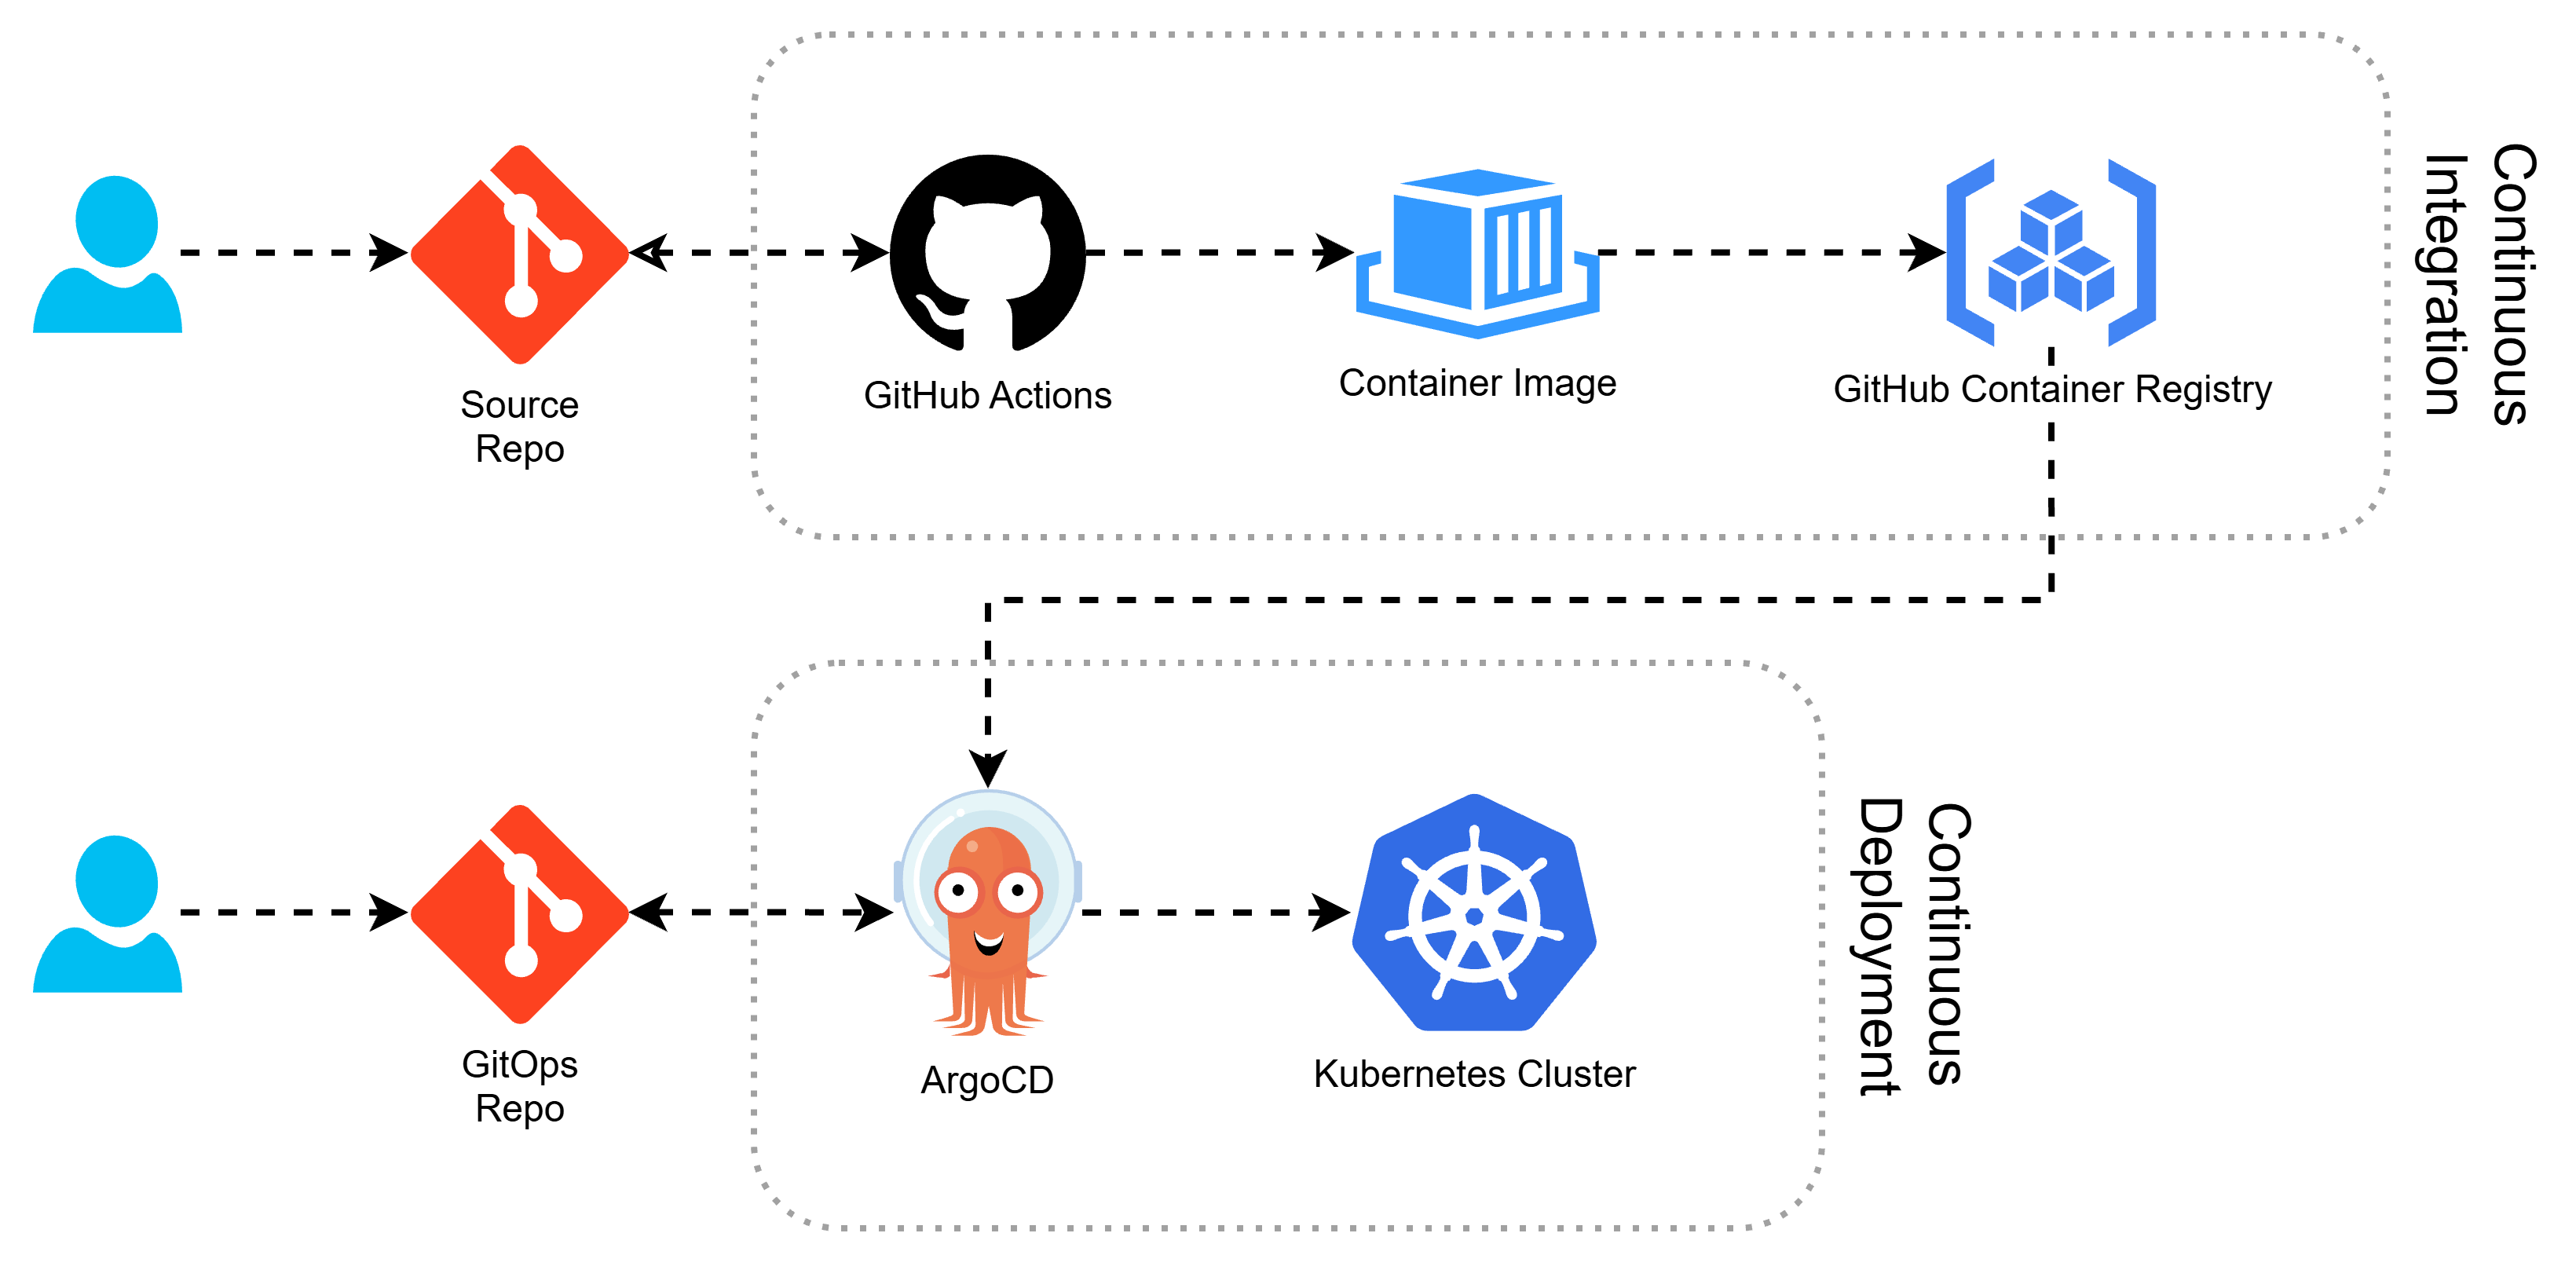
\includegraphics[width=0.8\textwidth,keepaspectratio]{images/pipeline-cicd.png}
            \end{figure}

            \begin{enumerate}[label=\alph*.]
                  \item \textit{Packaging} \textit{backend} dan \textit{frontend} ke dalam \textit{image} kontainer terpisah menggunakan \textit{multi-stage build}. \textit{Image} \textit{backend} dibangun dengan FrankenPHP serta Supervisor untuk manajemen proses, dengan berbagai mode kontainer seperti \texttt{server}, \texttt{horizon}, dan \texttt{scheduler}. \textit{Image} \textit{frontend} dibangun dengan konfigurasi mode keluaran \textit{standalone} Next.js dan dijalankan menggunakan \textit{runtime} Bun. Kode program dapat dilihat pada \annexref{annex:code-backend-dockerfile-file} dan \annexref{annex:code-frontend-dockerfile-file}.
                  \item \textit{Pipeline} CI menggunakan GitHub Actions yang mencakup tahapan validasi \textit{branch} dan versi, pembuatan dokumentasi API otomatis dengan Scribe, pembuatan \textit{changelog} melalui \textit{conventional commits}, pembangunan \textit{image} kontainer, penandatanganan \textit{image} dengan Cosign, dan rilis ke GitHub Container Registry. Kedua \textit{image} dibangun untuk multi-arsitektur (\texttt{linux/amd64} dan \texttt{linux/arm64}). Kode program \textit{pipeline} dapat dilihat pada \annexref{annex:code-backend-pipeline-file} dan \annexref{annex:code-frontend-pipeline-file}.
                  \item \textit{Deployment} di Kubernetes dikelola menggunakan pendekatan GitOps dengan ArgoCD, seperti yang dapat dilihat pada \annexref{annex:deployment-argocd}. Repositori Git berfungsi sebagai sumber kebenaran tunggal untuk seluruh konfigurasi infrastruktur deklaratif. ArgoCD secara kontinu memantau repositori Git dan menyinkronkan klaster Kubernetes agar sesuai dengan konfigurasi yang didefinisikan, termasuk deteksi penyimpangan (\textit{drift}) dan \textit{rollback} otomatis.
            \end{enumerate}

      \item Pengujian Kualitas Sistem

            Pengujian kualitas sistem informasi organisasi INFINITE dilakukan berdasarkan standar ISO/IEC 25010:2023 untuk \textit{Product Quality} dan ISO/IEC 25019:2023 untuk \textit{Quality in Use}, dengan empat karakteristik utama yang dipilih, yaitu \textit{Functional Suitability}, \textit{Interaction Capability}, \textit{Performance Efficiency}, dan \textit{Beneficialness}.
\end{enumerate}

\subsection{Cara Kerja Sistem Informasi}

Sistem informasi organisasi INFINITE terdiri dari dua komponen utama yang saling terintegrasi, yaitu \textit{backend} API Laravel dan \textit{frontend} Next.js. Sistem menyediakan autentikasi terpusat melalui protokol OIDC dengan sistem SSO INFINITE berbasis \textit{software} Authentik. \textit{Backend} menyediakan RESTful API berversi (\texttt{/api/v1/}) yang dikonsumsi oleh \textit{frontend} menggunakan \textit{library} Axios. Seluruh data dikomunikasikan dalam format JSON dengan paginasi berbasis kursor. Sistem dikelola melalui antarmuka dasbor web yang hanya dapat diakses oleh pengguna terautentikasi dengan peran dan hak akses yang sesuai.

\subsubsection{Manajemen Data Umum}

Manajemen data untuk setiap entitas secara umum mencakup pengelolaan informasi berupa pengaksesan, penambahan, pembaruan, dan penghapusan data. Pengguna dengan hak akses yang sesuai dengan data tertentu yang hendak dikelola dapat melakukan operasi tersebut melalui antarmuka dasbor web. Alur manajemen data secara umum dapat dilihat seperti pada \figref{fig:flow-manajemen-data-umum-diagram}.

\begin{figure}[H]
      \centering
      \caption{\textit{Flowchart} Manajemen Data Umum}
      \label{fig:flow-manajemen-data-umum-diagram}
      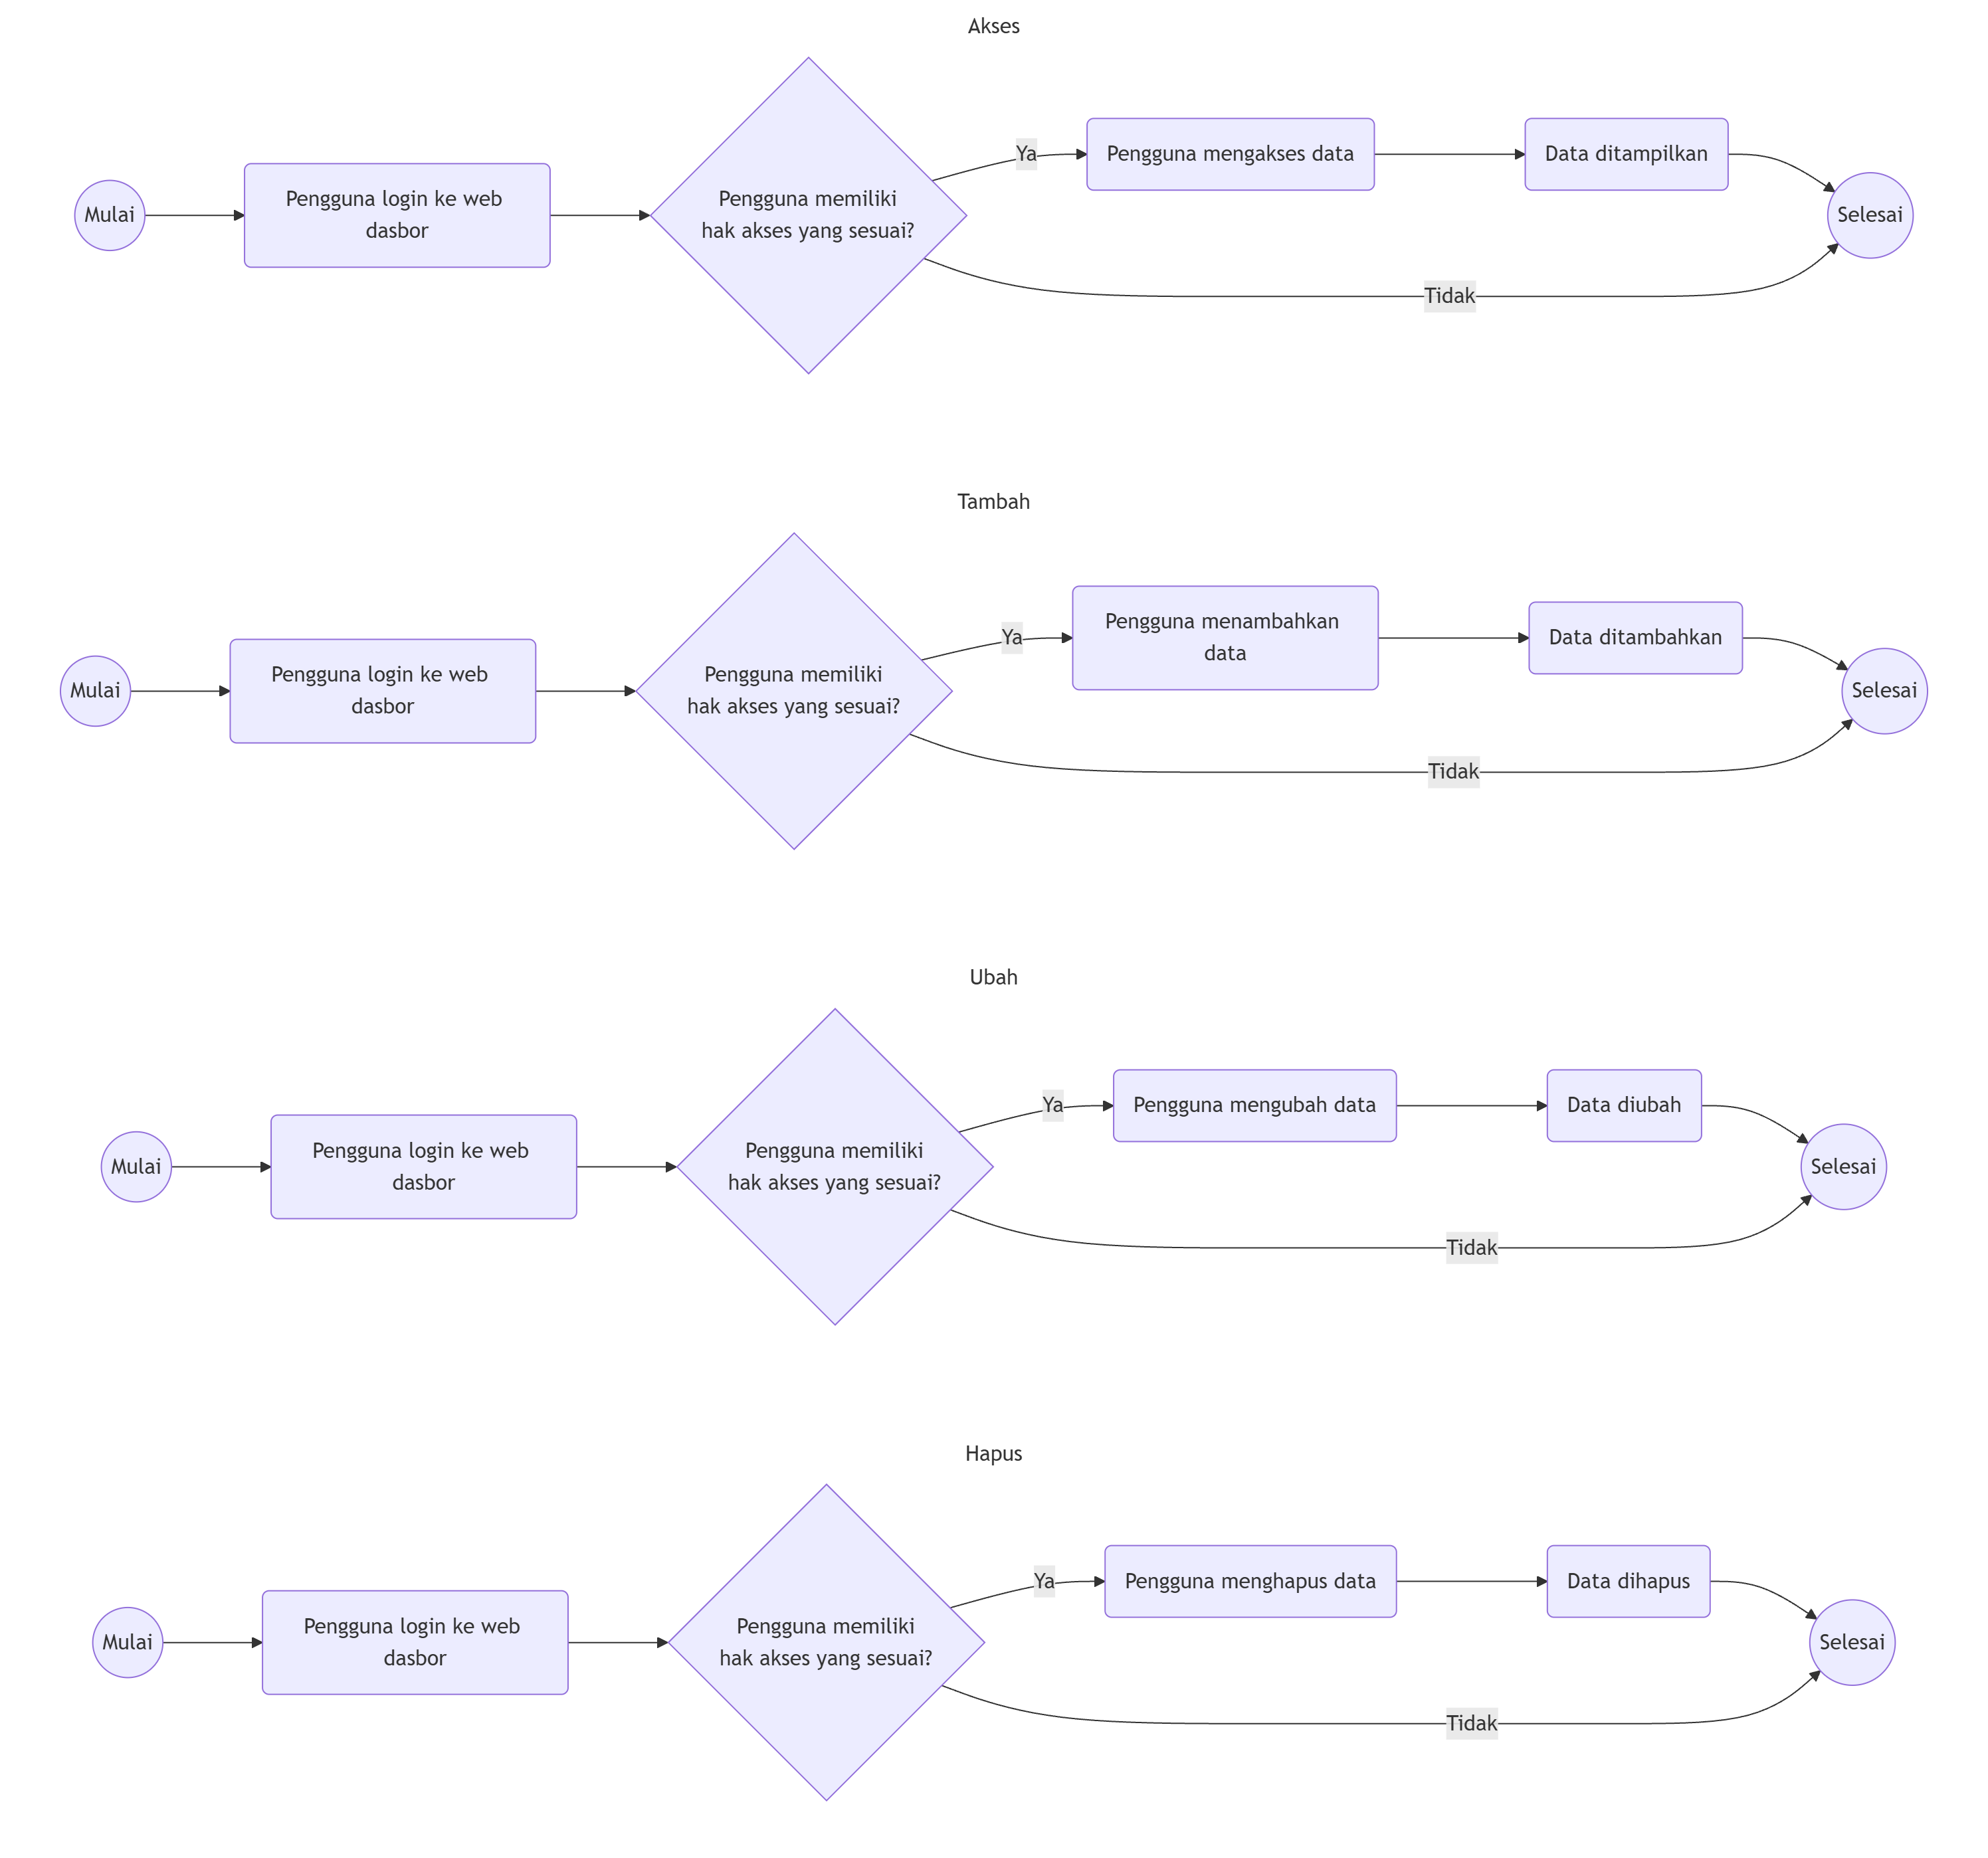
\includegraphics[width=1\textwidth,keepaspectratio]{images/umls/flow-manajemen-data-umum-diagram.png}
\end{figure}

\subsubsection{Manajemen Data Anggota}

Manajemen data anggota hampir serupa dengan manajemen data umum, namun memiliki alur tambahan untuk penentuan status keaktifan anggota, serta sinkronisasi profil ke sistem SSO INFINITE. Setiap anggota memiliki atribut \texttt{end\_date} yang menandai akhir masa aktif keanggotaan. Sistem secara otomatis menentukan status keaktifan anggota dengan membandingkan tanggal saat ini dengan tanggal \texttt{end\_date}. Jika tanggal saat ini melewati tanggal \texttt{end\_date}, maka status anggota menjadi tidak aktif (\texttt{is\_active = false}). Selain itu, setiap perubahan data anggota akan disinkronkan ke sistem SSO INFINITE melalui API Authentik untuk memastikan konsistensi data pengguna di seluruh sistem. Alur manajemen data anggota dapat dilihat seperti pada \figref{fig:flow-manajemen-data-anggota-diagram}.

\begin{figure}[H]
      \centering
      \caption{\textit{Flowchart} Manajemen Data Anggota}
      \label{fig:flow-manajemen-data-anggota-diagram}
      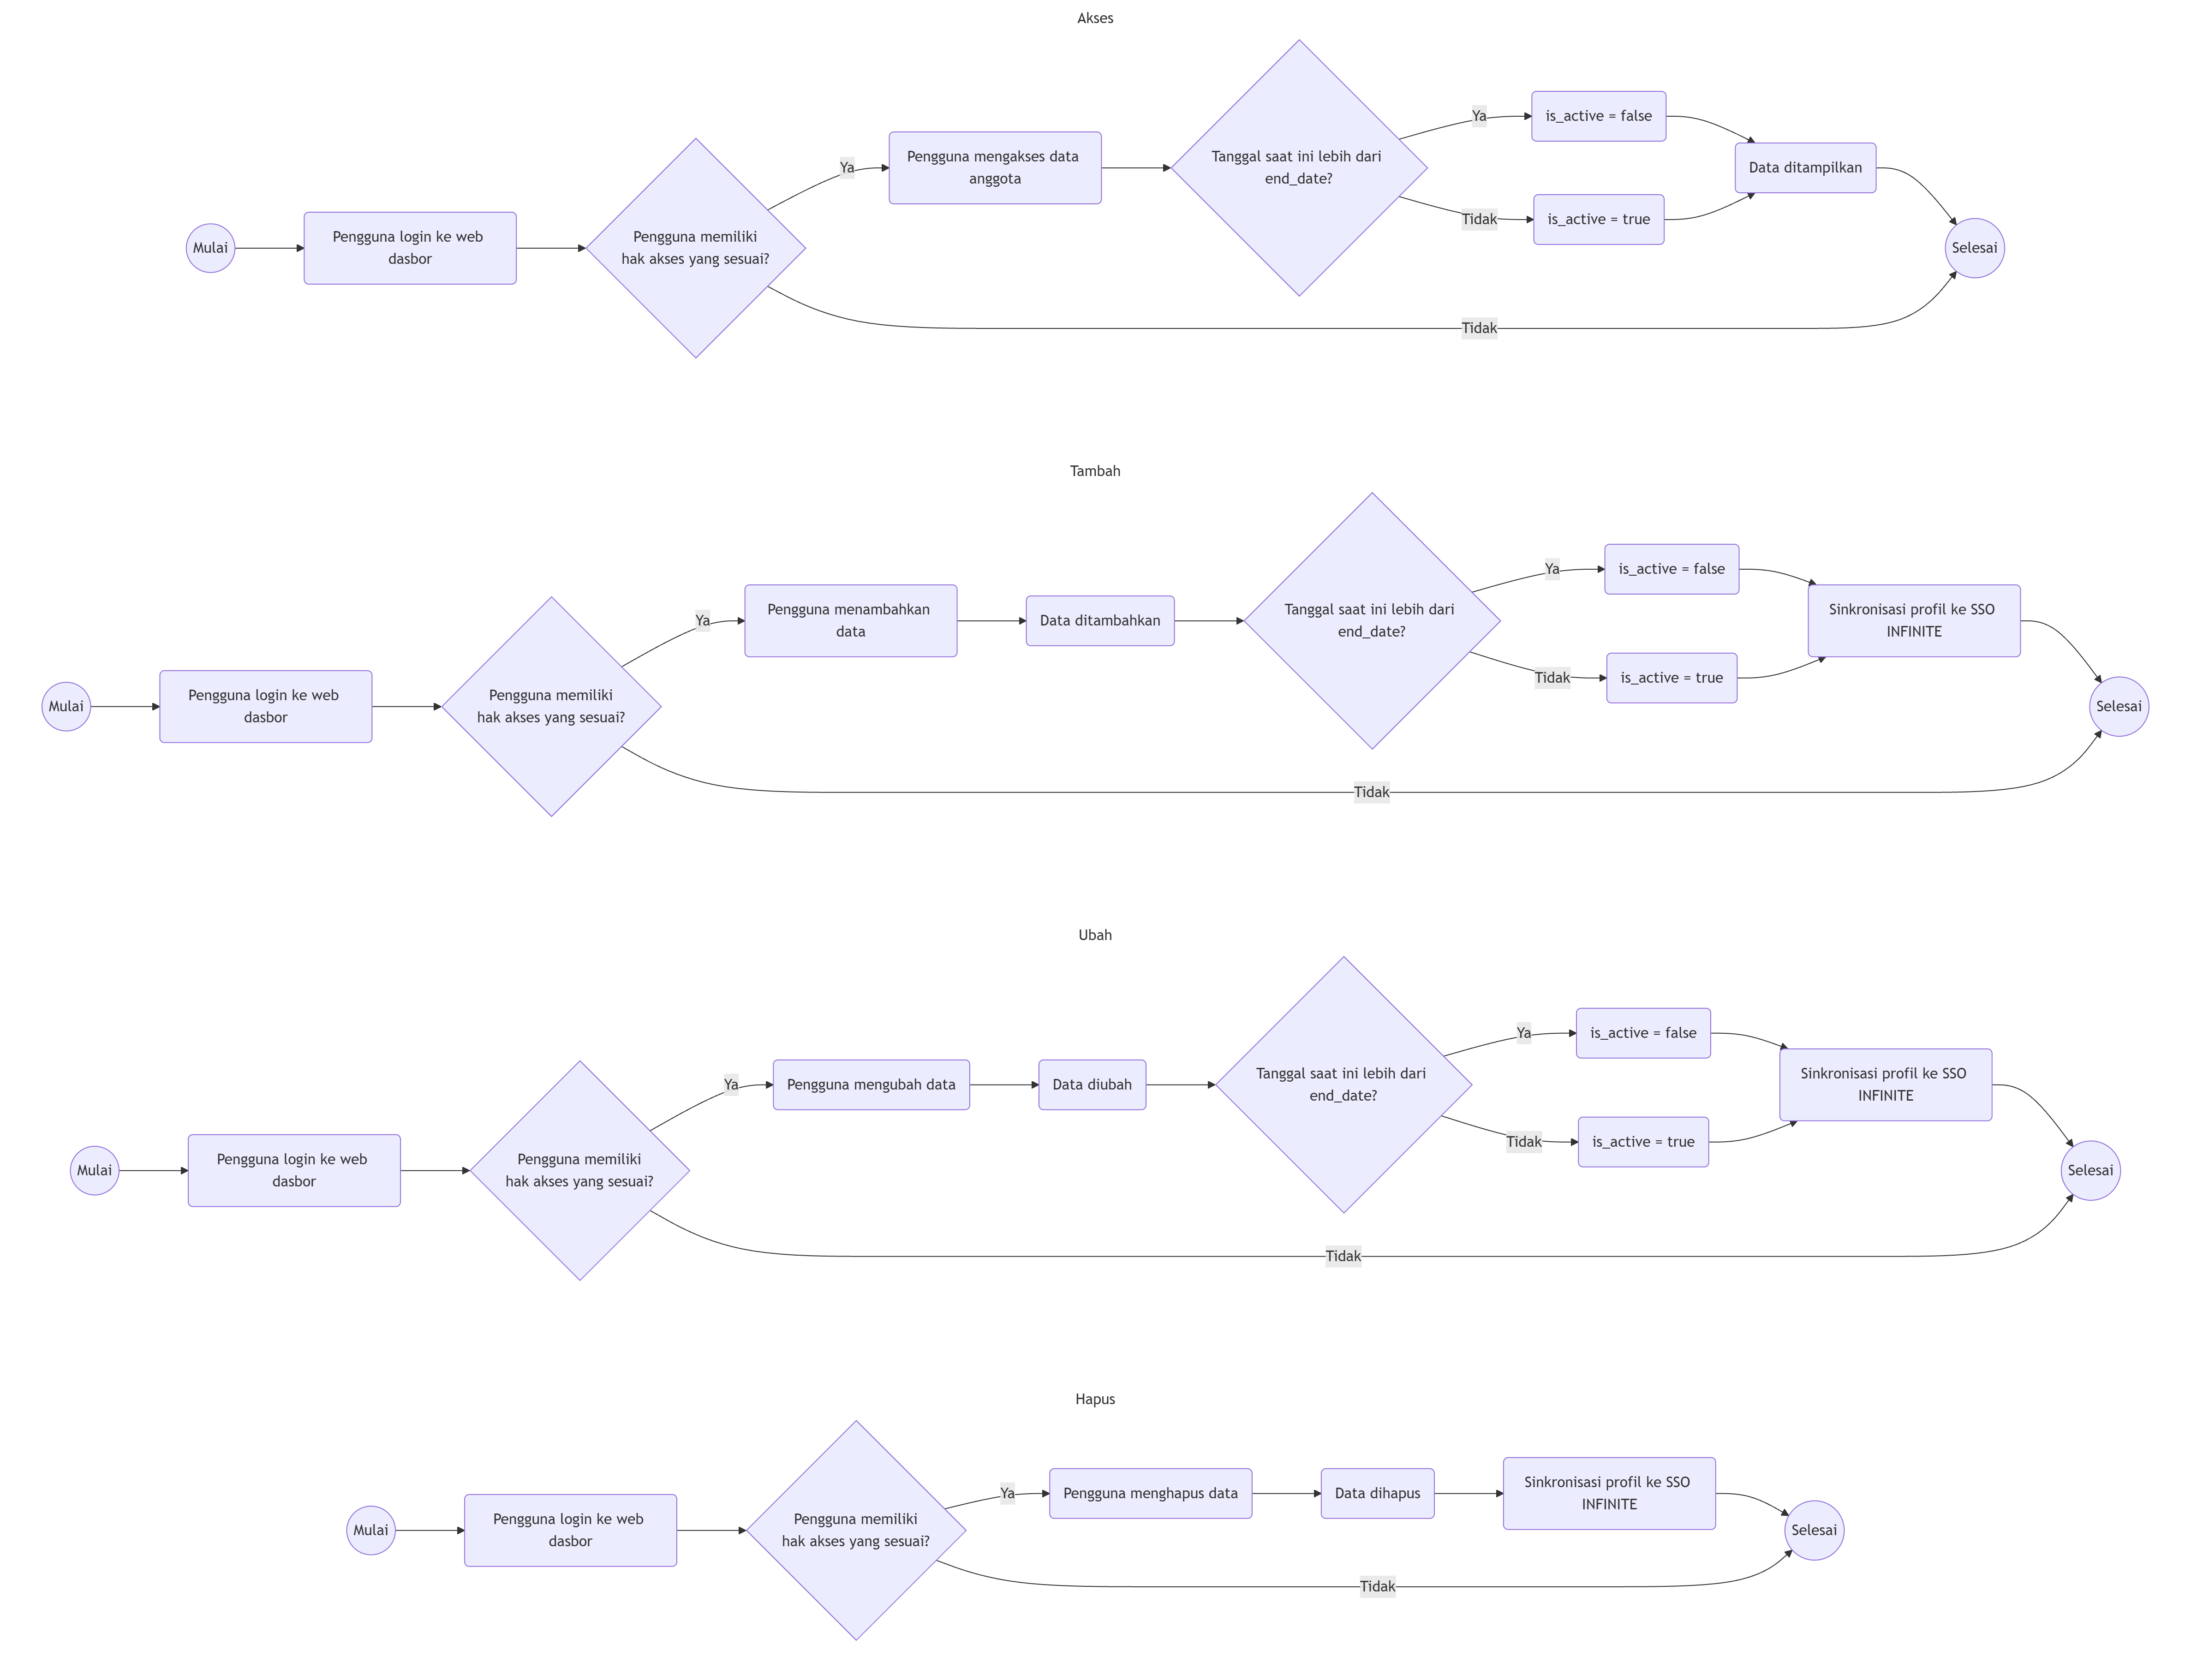
\includegraphics[width=1\textwidth,keepaspectratio]{images/umls/flow-manajemen-data-anggota-diagram.png}
\end{figure}

\subsubsection{Manajemen Data Kepengurusan}

Manajemen data kepengurusan mencakup pengelolaan struktur \textit{Core Team} dan \textit{Community Group Administrator}. Prosesnya juga hampir serupa dengan manajemen data umum, namun memiliki alur tambahan untuk penentuan kepengurusan yang aktif menjabat saat ini. Setiap waktu, hanya satu kepengurusan yang dapat aktif menjabat, sehingga setiap perubahan kepengurusan akan menonaktifkan kepengurusan sebelumnya. Setelah suatu periode kepengurusan dibuat, pengguna kemudian dapat menetapkan anggota yang mengisi posisi di setiap divisi atau grup.

\subsubsection{Manajemen Data Kompetisi}

Manajemen data kompetisi dimulai dari pengelolaan data \texttt{Competition} sebagai induk katalog. Untuk setiap tahun atau edisi pelaksanaan kompetisi, dicatatkan sebuah \texttt{CompetitionInstance} baru yang merujuk pada induk katalog kompetisi, dilengkapi dengan informasi spesifik pelaksanaan seperti penyelenggara, tanggal, lokasi, dan tautan. Taksonomi kompetisi seperti tipe penyelenggara, tingkat kompetisi, peringkat, durasi, jenis luaran, dan tipe tim didefinisikan sebagai data referensi terpisah yang masing-masing memiliki bobot penilaian.

\subsubsection{Manajemen Data Pendanaan dan Prestasi Tim}

Pengguna membentuk \texttt{Team} untuk mengikuti kompetisi, dengan menunjuk salah satu pengguna sebagai ketua tim dan menambahkan pengguna lainnya sebagai anggota tim. Pengajuan \texttt{FundApplication} diajukan oleh tim yang telah dinyatakan lolos seleksi suatu kompetisi dan membutuhkan pendanaan untuk melanjutkan ke tahap berikutnya. Proses pengajuan dilengkapi dengan pengunggahan dokumen bukti lolos seleksi dan proposal pendanaan yang disimpan dalam bentuk PDF. Pengajuan berada dalam status \texttt{Pending} pada awalnya, kemudian dapat diterima (\texttt{Accepted}) atau ditolak (\texttt{Rejected}) oleh pengurus dengan hak akses yang sesuai. Setiap perubahan status dapat dilihat oleh pemohon.

Setelah kompetisi dilaksanakan, \texttt{Achievement} dicatat dengan mencantumkan tim beserta data-data kompetisi dan taksonomi lainnya yang sesuai. Sistem secara otomatis menghitung poin prestasi berdasarkan perkalian bobot keenam taksonomi (\texttt{organizer\_type} $\times$ \texttt{team\_type} $\times$ \texttt{scale} $\times$ \texttt{time\_range} $\times$ \texttt{output} $\times$ \texttt{rank}). Poin-poin ini kemudian diakumulasi ke dalam \texttt{AchievementLeaderboard} yang menampilkan peringkat anggota per tahun berdasarkan total poin.

\subsubsection{Manajemen Data Grup dan Hak Akses}

Manajemen data grup dan hak akses dilakukan melalui pengelolaan \texttt{Group} dan \texttt{Permission}, yang juga hampir serupa dengan manajemen data umum. Setiap grup memiliki daftar hak akses yang ditetapkan, dan setiap pengguna dapat menjadi anggota dari satu atau beberapa grup. Sistem secara otomatis menentukan hak akses pengguna berdasarkan gabungan hak akses dari semua grup yang diberikan. Pengguna dengan hak akses yang sesuai dapat menambahkan atau menghapus anggota. Secara bawaan, setiap pengguna yang merupakan anggota INFINITE akan menjadi anggota grup \texttt{Member}, sedangkan pengurus akan menjadi anggota grup \texttt{Core Team xxxx} atau \texttt{CG Admin xxxx} sesuai dengan periode kepengurusan masing-masing. Anggota yang aktif akan diberikan pula grup \texttt{Active Member}, sedangkan anggota yang tidak aktif akan diberikan grup \texttt{Inactive Member}. Sedangkan pengurus yang aktif menjabat akan diberikan grup \texttt{Core Team} atau \texttt{CG Admin}, sedangkan pengurus yang tidak aktif menjabat akan diberikan grup \texttt{Ex Core Team} atau \texttt{Ex CG Admin}.

\subsubsection{Manajemen Konfigurasi}

Manajemen konfigurasi dilakukan melalui halaman \textit{Settings} pada web dasbor, dan disimpan dalam tabel \texttt{Configs} berupa pasangan kunci-nilai dengan tipe data dan penanda privasi. Konfigurasi publik dapat diakses melalui endpoint API tanpa autentikasi, sedangkan konfigurasi privat hanya tersedia untuk pengguna terautentikasi. Konfigurasi hanya dapat dikelola oleh pengguna dengan izin yang sesuai.

\subsection{Kualitas Sistem Informasi}

Pengujian kualitas sistem informasi dilakukan setelah semua komponen individu saling terintegrasi menjadi satu kesatuan sistem yang utuh. Pengujian kualitas dilakukan mengacu pada standar ISO/IEC 25010:2023 untuk \textit{Product Quality} dan ISO/IEC 25019:2023 untuk \textit{Quality in Use}, dengan empat karakteristik yang dievaluasi, yaitu \textit{Functional Suitability}, \textit{Interaction Capability}, \textit{Performance Efficiency}, dan \textit{Beneficialness}.

Aspek \textit{Functional Suitability} dan \textit{Interaction Capability} yang termasuk dalam aspek \textit{Product Quality} diuji oleh lima tenaga ahli dalam bidang sistem informasi. Kelima tenaga ahli memiliki latar belakang dan pemahaman yang memadai baik secara profesional maupun terkait INFINITE. Identitas kelima tenaga ahli dapat dilihat pada \tabref{tab:tenaga-ahli-penguji}.

\begin{table}[H]
      \centering
      \setstretch{1.2}
      \caption{Identitas Tenaga Ahli Penguji}
      \label{tab:tenaga-ahli-penguji}
      \begin{tabular}{|c|p{4cm}|p{3cm}|p{4cm}|}
            \hline
            \textbf{No.} & \textbf{Nama}                          & \textbf{Profesi}                  & \textbf{Instansi}             \\
            \hline
            1            & Ikhwan Inzaghi                         & \textit{Software Engineer}
                         & Universitas Nahdlatul Ulama Yogyakarta                                                                     \\
            \hline
            2            & Zainal Ma'ruf Abidin                   & UI/UX \textit{Designer}           & PT Digdaya Inovasi Gemilang
            \\
            \hline
            3            & Damar Albaribin Syamsu                 & AI \textit{Software Engineer}     & Pelgo Incorporated            \\
            \hline
            4            & Satya Adhiyaksa Ardy                   & \textit{System Software Engineer} & Sillicon XPandas              \\
            \hline
            5            & Dzul Fadli Rahman, S.Kom., M.Sc.       & Dosen                             & Universitas Negeri Yogyakarta
            \\
            \hline
      \end{tabular}
\end{table}

Aspek \textit{Performance Efficiency} diuji menggunakan Google Lighthouse untuk \textit{frontend} dan Grafana k6 untuk \textit{backend}. Sedangkan aspek \textit{Beneficialness} diuji oleh sembilan pengurus dan sembilan anggota INFINITE.

\subsubsection{Hasil Pengujian \textit{Functional Suitability}}

Pengujian \textit{Functional Suitability} dilakukan untuk memastikan kesesuaian seluruh fungsi utama sistem dengan spesifikasi yang diharapkan. Hasil pengujian  yang telah dilakukan oleh lima tenaga ahli dapat dilihat pada \annexref{annex:product-quality}. Berikut adalah ringkasan hasil pengujiannya:

\begin{table}[H]
      \centering
      \setstretch{1.2}
      \caption{Skor Pengujian \textit{Functional Suitability}}
      \label{tab:skor-functional-suitability}
      \begin{tabular}{|c|p{8cm}|c|}
            \hline
            \textbf{No.}                         & \textbf{Nama Penguji}            & \textbf{Skor} \\
            \hline
            1                                    & Ikhwan Inzaghi                   & 23            \\
            \hline
            2                                    & Zainal Ma'ruf Abidin             & 23            \\
            \hline
            3                                    & Damar Albaribin Syamsu           & 23            \\
            \hline
            4                                    & Satya Adhiyaksa Ardy             & 23            \\
            \hline
            5                                    & Dzul Fadli Rahman, S.Kom., M.Sc. & 23            \\
            \hline
            \multicolumn{2}{|c|}{\textbf{Total}} & \textbf{115}                                     \\
            \hline
      \end{tabular}
\end{table}

Dari total skor tersebut, kemudian dilakukan perhitungan sesuai dengan rumus persentase kelayakan pada \equref{eq:functional_suitability}, sehingga diperoleh:

\begin{equation}
      \text{Persentase Kelayakan} = \frac{115}{23 \times 5 \times 1} \times 100\% = \frac{115}{115} \times 100\% = 100\%
\end{equation}

Berdasarkan kriteria interpretasi kelayakan pada \tabref{tab:kriteria_functional}, hasil pengujian \textit{Functional Suitability} sebesar 100\% termasuk dalam kriteria \textbf{Sangat Layak}, yang menunjukkan bahwa seluruh fungsi sistem telah berjalan sesuai dengan spesifikasi yang diharapkan.

\subsubsection{Hasil Pengujian \textit{Interaction Capability}}

Pengujian \textit{Interaction Capability} dilakukan menggunakan \textit{USE Questionnaire} yang mencakup empat dimensi, yaitu \textit{Usefulness}, \textit{Ease of Use}, \textit{Ease of Learning}, dan \textit{Satisfaction}. Pengujian ini bertujuan untuk mengukur dan memastikan aspek kegunaan, kemudahan penggunaan, kemudahan pembelajaran, dan kepuasan pengguna. Hasil pengujian  yang telah dilakukan oleh lima tenaga ahli dapat dilihat pada \annexref{annex:product-quality}. Berikut adalah ringkasan hasil pengujiannya:

\begin{table}[H]
      \centering
      \setstretch{1.2}
      \caption{Skor Pengujian \textit{Interaction Capability}}
      \label{tab:skor-interaction-capability}
      \begin{tabular}{|c|p{8cm}|c|}
            \hline
            \textbf{No.}                         & \textbf{Nama Penguji}            & \textbf{Skor} \\
            \hline
            1                                    & Ikhwan Inzaghi                   & 122           \\
            \hline
            2                                    & Zainal Ma'ruf Abidin             & 133           \\
            \hline
            3                                    & Damar Albaribin Syamsu           & 150           \\
            \hline
            4                                    & Satya Adhiyaksa Ardy             & 136           \\
            \hline
            5                                    & Dzul Fadli Rahman, S.Kom., M.Sc. & 147           \\
            \hline
            \multicolumn{2}{|c|}{\textbf{Total}} & \textbf{688}                                     \\
            \hline
      \end{tabular}
\end{table}

Dari total skor tersebut, kemudian dilakukan perhitungan sesuai dengan rumus persentase kelayakan pada \equref{eq:interaction_capability_satisfaction}, sehingga diperoleh:

\begin{equation}
      \text{Persentase Kelayakan} = \frac{688}{30 \times 5 \times 5} \times 100\% = \frac{688}{750} \times 100\% = 91{,}73\%
\end{equation}

Berdasarkan kriteria interpretasi kelayakan pada \tabref{tab:kriteria_interaction_capability_satisfaction}, hasil pengujian \textit{Interaction Capability} sebesar 91{,}73\% termasuk dalam kriteria \textbf{Sangat Layak}, yang menunjukkan bahwa sistem informasi memiliki tingkat kegunaan, kemudahan penggunaan, kemudahan pembelajaran, dan kepuasan pengguna yang sangat baik.

\subsubsection{Hasil Pengujian \textit{Performance Efficiency}}

Pengujian \textit{Performance Efficiency} bertujuan untuk mengukur performa sistem informasi INFINITE dalam merespons permintaan pengguna dan memproses data. Pengujiann ini dilakukan dengan dua pendekatan:
\begin{enumerate}[label=\alph*.]
      \item Pengujian \textit{frontend} Next.js dilakukan menggunakan Google Lighthouse pada seluruh halaman web dasbor. Hasil pengujian lengkap dapat dilihat pada \annexref{annex:performance-frontend}. Berdasarkan hasil tersebut, didapatkan rata-rata skor performa \textit{frontend} sebesar 90,42, yang termasuk dalam kategori \textbf{Baik} menurut kriteria interpretasi skor performa Lighthouse pada \tabref{tab:kriteria_lighthouse}.
      \item Pengujian \textit{backend} API Laravel dilakukan menggunakan Grafana k6 dengan tipe \textit{breakpoint test}. Pengujian dilakukan pada \textit{endpoint} utama API untuk menemukan batas kapasitas sistem. Hasil pengujian lengkap dapat dilihat pada \annexref{annex:performance-backend}. Berdasarkan hasil tersebut, didapatkan rata-rata \textit{Response Time} sebesar \textbf{1 detik}, rata-rata \textit{Throughput} sebesar \textbf{53,6 permintaan per detik}, dan rata-rata \textit{Error Rate} sebesar \textbf{0\%}, serta maksimum jumlah \textit{Virtual Users} sebanyak \textbf{189 pengguna simultan}.
\end{enumerate}

\subsubsection{Hasil Pengujian \textit{Beneficialness}}

Pengujian \textit{Beneficialness} dilakukan menggunakan kuesioner \textit{End-User Computing Satisfaction} (EUCS) yang mencakup lima dimensi, yaitu \textit{Content}, \textit{Accuracy}, \textit{Format}, \textit{Ease of Use}, dan \textit{Timeliness}. Pengujian ini bertujuan untuk mengukur dan memastikan kemanfaatan sistem informasi INFINITE bagi pengguna akhir. Berikut adalah ringkasan hasil pengujiannya:
\begin{table}[H]
      \centering
      \setstretch{1.2}
      \caption{Skor Pengujian \textit{Beneficialness}}
      \label{tab:skor-satisfaction}
      \fontsize{8}{10}\selectfont
      \begin{tabular}{|c|c|c|c|c|c|c|c|c|c|c|c|c|c|c|}
            \hline
            \textbf{No.}                          & \textbf{Nama} & \textbf{Q1} & \textbf{Q2} & \textbf{Q3} & \textbf{Q4} & \textbf{Q5} & \textbf{Q6} & \textbf{Q7} & \textbf{Q8} & \textbf{Q9} & \textbf{Q10} & \textbf{Q11} & \textbf{Q12} & \textbf{Total} \\
            \hline
            1                                     & Pengurus 1    & 4           & 4           & 4           & 4           & 5           & 5           & 2           & 4           & 2           & 4            & 2            & 4            & 44             \\
            \hline
            2                                     & Pengurus 2    & 4           & 4           & 5           & 5           & 5           & 5           & 5           & 5           & 4           & 4            & 4            & 4            & 54             \\
            \hline
            3                                     & Pengurus 3    & 5           & 4           & 5           & 5           & 5           & 5           & 5           & 5           & 5           & 3            & 5            & 4            & 56             \\
            \hline
            4                                     & Pengurus 4    & 4           & 4           & 4           & 4           & 4           & 4           & 4           & 4           & 4           & 4            & 4            & 4            & 48             \\
            \hline
            5                                     & Pengurus 5    & 4           & 4           & 4           & 4           & 4           & 4           & 4           & 4           & 4           & 4            & 4            & 4            & 48             \\
            \hline
            6                                     & Pengurus 6    & 4           & 3           & 3           & 4           & 4           & 3           & 3           & 4           & 3           & 4            & 4            & 3            & 42             \\
            \hline
            7                                     & Pengurus 7    & 5           & 5           & 5           & 5           & 5           & 5           & 5           & 5           & 5           & 5            & 5            & 5            & 60             \\
            \hline
            8                                     & Pengurus 8    & 3           & 3           & 3           & 3           & 4           & 4           & 4           & 4           & 4           & 4            & 4            & 4            & 44             \\
            \hline
            9                                     & Pengurus 9    & 4           & 4           & 4           & 4           & 4           & 4           & 4           & 4           & 4           & 4            & 4            & 4            & 48             \\
            \hline
            10                                    & Anggota 1     & 5           & 5           & 5           & 5           & 5           & 5           & 5           & 5           & 5           & 5            & 5            & 5            & 60             \\
            \hline
            11                                    & Anggota 2     & 3           & 4           & 4           & 3           & 4           & 4           & 3           & 3           & 3           & 4            & 3            & 4            & 42             \\
            \hline
            12                                    & Anggota 3     & 4           & 4           & 3           & 4           & 4           & 4           & 4           & 4           & 2           & 2            & 2            & 4            & 41             \\
            \hline
            13                                    & Anggota 4     & 4           & 4           & 4           & 4           & 4           & 4           & 4           & 4           & 4           & 4            & 4            & 4            & 48             \\
            \hline
            14                                    & Anggota 5     & 4           & 4           & 4           & 4           & 4           & 4           & 4           & 3           & 4           & 4            & 3            & 4            & 46             \\
            \hline
            15                                    & Anggota 6     & 5           & 4           & 5           & 5           & 4           & 5           & 4           & 5           & 5           & 4            & 3            & 5            & 54             \\
            \hline
            16                                    & Anggota 7     & 4           & 4           & 3           & 4           & 4           & 4           & 4           & 5           & 4           & 4            & 3            & 4            & 47             \\
            \hline
            17                                    & Anggota 8     & 4           & 4           & 4           & 3           & 5           & 4           & 4           & 4           & 4           & 4            & 4            & 4            & 48             \\
            \hline
            18                                    & Anggota 9     & 4           & 4           & 4           & 4           & 4           & 4           & 4           & 4           & 4           & 4            & 4            & 4            & 48             \\
            \hline
            \multicolumn{14}{|c|}{\textbf{Total}} & \textbf{878}                                                                                                                                                                                              \\
            \hline
      \end{tabular}
\end{table}

Dari total skor tersebut, kemudian dilakukan perhitungan sesuai dengan rumus persentase kelayakan pada \equref{eq:interaction_capability_satisfaction}, sehingga diperoleh:

\begin{equation}
      \text{Persentase Kelayakan} = \frac{878}{12 \times 5 \times 18} \times 100\% = \frac{878}{1080} \times 100\% = 81{,}30\%
\end{equation}

Berdasarkan kriteria interpretasi kelayakan pada \tabref{tab:kriteria_interaction_capability_satisfaction}, hasil pengujian \textit{Beneficialness} sebesar 81{,}30\% termasuk dalam kriteria \textbf{Sangat Layak}, yang menunjukkan bahwa sistem informasi memberikan kemanfaatan yang sangat baik bagi pengguna akhir.

\section{Pembahasan}

Sistem informasi organisasi INFINITE dikembangkan untuk mengatasi permasalahan-permasalahan yang dihadapi sistem yang telah ada sebelumnya sebagaimana diidentifikasi pada latar belakang penelitian, yaitu: (1)~sistem informasi yang terpecah dalam dua sistem berupa sistem Laravel di \textit{shared hosting} dan sistem Strapi di server terpisah, menciptakan fragmentasi dan potensi inkonsistensi data; (2)~sistem Strapi yang tidak mendukung integrasi dengan protokol OIDC untuk memungkinkan autentikasi terpusat dengan sistem SSO; (3)~sistem Laravel yang tidak memiliki \textit{image} kontainer untuk dapat di-\textit{deploy} pada platform Kubernetes; (4)~pengoperasian dua infrastruktur secara bersamaan (\textit{shared hosting} dan VPS) yang mengakibatkan inefisiensi biaya operasional; serta (5)~sistem Laravel yang menggunakan arsitektur \textit{monolithic} sehingga tidak menyediakan API untuk integrasi dengan aplikasi lain. Sistem baru ini dikembangkan menggunakan model \textit{Waterfall} yang terdiri dari empat tahapan pelaksanaan, yaitu \textit{Requirements Definition}, \textit{System and Software Design}, \textit{Implementation and Unit Testing}, serta \textit{Integration and System Testing}. Tahap pertama dimulai dengan analisis kebutuhan melalui wawancara dengan pengurus INFINITE dan observasi terhadap sistem informasi yang telah ada sebelumnya. Hasil analisis dijadikan sebagai acuan untuk merancang arsitektur sistem, antarmuka pengguna, serta basis data. Rancangan kemudian diimplementasikan menggunakan Laravel sebagai \textit{backend} dengan arsitektur \textit{headless}, dan Next.js sebagai \textit{frontend}. Implementasi menghasilkan sistem informasi organisasi INFINITE yang terintegrasi dengan autentikasi OIDC SSO INFINITE dan di-\textit{deploy} sebagai aplikasi terkontainerisasi di Kubernetes.

Sistem informasi yang dihasilkan menyederhakan proses administrasi dan pengelolaan informasi organisasi INFINITE. Data organisasi yang sebelumnya terfragmentasi dalam sistem monolitik di \textit{shared hosting} dan Strapi di dua server terpisah kini menjadi satu platform terintegrasi yang terkontainerisasi dan ter-\textit{deploy} di Kubernetes. Konsolidasi infrastruktur ini sekaligus mengatasi inefisiensi biaya operasional karena kebutuhan \textit{shared hosting} tersendiri tidak lagi diperlukan. Selain itu, integrasi autentikasi OIDC dengan sistem SSO INFINITE juga menyelesaikan tantangan fragmentasi autentikasi yang sebelumnya dihadapi. Seluruh aplikasi dalam ekosistem INFINITE kini dapat menggunakan satu set kredensial tunggal, meningkatkan pengalaman pengguna dan mengurangi beban administratif dalam pengelolaan akun.

Arsitektur \textit{headless} yang diterapkan pada sistem informasi INFINITE memberikan beberapa keunggulan signifikan dibandingkan sistem monolitik sebelumnya. Pertama, pemisahan total antara \textit{backend} dan \textit{frontend} memungkinkan kedua komponen dikembangkan, di-\textit{deploy}, dan diskalakan secara independen. Hal ini sejalan dengan kebutuhan INFINITE yang beroperasi di lingkungan Kubernetes, di mana setiap komponen berjalan dalam kontainer terpisah yang dapat diskalakan sesuai beban. Kedua, pendekatan API-\textit{first} memungkinkan \textit{backend} untuk tidak hanya melayani \textit{frontend} utama, tetapi juga menyediakan API yang dapat dikonsumsi oleh aplikasi-aplikasi lain dalam ekosistem INFINITE. Ketiga, penggunaan \textit{Clean Architecture} pada \textit{frontend} Next.js meningkatkan modularitas dan memudahkan pemeliharaan, dengan pemisahan tegas antara domain, aplikasi, infrastruktur, dan presentasi.

Penggunaan model \textit{deployment} dengan kontainer dan lingkungan Kubernetes juga memberikan fleksibilitas, skalabilitas, dan konsistensi yang lebih baik. \textit{Pipeline} CI/CD berbasis GitHub Actions memastikan bahwa setiap perubahan kode pada \textit{backend} dan \textit{frontend} melalui proses validasi, pembangunan \textit{image} kontainer, penandatanganan digital, dan rilis ke \textit{registry} yang terotomasi.  Pengelolaan Kubernetes melalui ArgoCD secara deklaratif dengan GitOps sebagai sumber kebenaran tunggal memastikan bahwa seluruh konfigurasi infrastruktur dapat direproduksi, dimonitor, disinkronkan, dideteksi dan dipulihkan dari penyimpangan (\textit{drift}), serta dilakukan \textit{rollback} secara otomatis.

Pengujian kualitas sistem berdasarkan standar ISO/IEC 25010:2023 untuk \textit{Product Quality} dan ISO/IEC 25019:2023 untuk \textit{Quality in Use} dilakukan untuk memvalidasi bahwa sistem yang dikembangkan memenuhi kebutuhan pengguna dan standar kualitas perangkat lunak. Pengujian dilakukan terhadap empat karakteristik, yaitu \textit{Functional Suitability}, \textit{Interaction Capability}, \textit{Performance Efficiency}, dan \textit{Beneficialness}, dengan hasil sebagai berikut:

\begin{enumerate}[label=\alph*.]
      \item Pengujian \textit{Functional Suitability} dilakukan oleh lima tenaga ahli dan memperoleh persentase kelayakan sebesar 100\% yang termasuk dalam kategori \textbf{Sangat Layak}. Hasil ini membuktikan bahwa seluruh fungsi sistem telah berjalan sesuai dengan spesifikasi yang diharapkan.
      \item Pengujian \textit{Interaction Capability} menggunakan \textit{USE Questionnaire} dilakukan oleh lima tenaga ahli dan memperoleh persentase kelayakan sebesar 91{,}73\% yang termasuk dalam kategori \textbf{Sangat Layak}. Hasil ini membuktikan bahwa sistem informasi memiliki tingkat kegunaan, kemudahan penggunaan, kemudahan pembelajaran, dan kepuasan pengguna yang sangat baik.
      \item Pengujian \textit{Performance Efficiency} dilakukan dengan dua pendekatan. Pengujian \textit{frontend} menggunakan Google Lighthouse memperoleh rata-rata skor performa sebesar 90{,}42 yang termasuk dalam kategori \textbf{Baik}. Hasil ini menunjukkan bahwa halaman-halaman dasbor \textit{frontend} dengan Next.js memiliki waktu pemuatan yang efisien dan memenuhi standar responsivitas aplikasi web modern. Pengujian \textit{backend} menggunakan Grafana k6 dengan tipe \textit{breakpoint test} memperoleh rata-rata \textit{Response Time} sebesar \textbf{1 detik}, rata-rata \textit{Throughput} sebesar \textbf{53{,}6 permintaan per detik}, rata-rata \textit{Error Rate} sebesar \textbf{0\%}, serta maksimum jumlah \textit{Virtual Users} sebanyak \textbf{189 pengguna simultan}. Hasil ini memvalidasi bahwa \textit{backend} yang dijalankan menggunakan Laravel Octane dengan FrankenPHP mampu menangani beban yang diantisipasi dengan respons yang cepat dan tanpa kesalahan.
      \item Pengujian \textit{Beneficialness} menggunakan kuesioner \textit{End-User Computing Satisfaction} (EUCS) dilakukan oleh sembilan pengurus dan sembilan anggota INFINITE serta memperoleh persentase kelayakan sebesar 81{,}30\% yang termasuk dalam kategori \textbf{Sangat Layak}. Hasil ini membuktikan bahwa sistem yang dikembangkan memberikan kemanfaatan yang sangat baik bagi pengguna, baik pengurus maupun anggota INFINITE.
\end{enumerate}

Berdasarkan hasil pengujian keempat karakteristik tersebut, dapat disimpulkan bahwa sistem informasi organisasi INFINITE yang dikembangkan berjalan dengan baik secara fungsional dan teknis, serta diterima dengan baik oleh pengguna. Sistem tergolong layak digunakan sebagai solusi dalam mendukung pengelolaan data organisasi INFINITE secara terintegrasi dan berkelanjutan.